% -*- Mode:TeX -*-

%% IMPORTANT: The official thesis specifications are available at:
%%            http://libraries.mit.edu/archives/thesis-specs/
%%
%%            Please verify your thesis' formatting and copyright
%%            assignment before submission.  If you notice any
%%            discrepancies between these templates and the 
%%            MIT Libraries' specs, please let us know
%%            by e-mailing thesis@mit.edu

%% The documentclass options along with the pagestyle can be used to generate
%% a technical report, a draft copy, or a regular thesis.  You may need to
%% re-specify the pagestyle after you \include  cover.tex.  For more
%% information, see the first few lines of mitthesis.cls. 

%\documentclass[12pt,vi,twoside]{mitthesis}
%%
%%  If you want your thesis copyright to you instead of MIT, use the
%%  ``vi'' option, as above.
%%
%\documentclass[12pt,twoside,leftblank]{mitthesis}
%%
%% If you want blank pages before new chapters to be labelled ``This
%% Page Intentionally Left Blank'', use the ``leftblank'' option, as
%% above. 

\documentclass[12pt,vi,twoside,leftblank]{mitthesis}
\usepackage{lgrind}
%% These have been added at the request of the MIT Libraries, because
%% some PDF conversions mess up the ligatures.  -LB, 1/22/2014
\usepackage{cmap}
\usepackage[T1]{fontenc}
\usepackage{amsmath}
\usepackage{amsthm}
\usepackage{amssymb}
\usepackage{amsfonts}
\usepackage{graphicx}
\usepackage{ftnxtra}
\usepackage{courier}
\usepackage{listings}
\lstset{showstringspaces=false}
\lstset{basicstyle=\footnotesize\ttfamily,breaklines=true}
\usepackage{multirow}
\usepackage{mathcomp}
\usepackage{subcaption}
%\usepackage{times}
%\usepackage{float}
\usepackage{hyperref}
\hypersetup{
    colorlinks=true,
    linkcolor=blue,
    citecolor = red,
}
\urlstyle{same}
\graphicspath{ {image/} }
\pagestyle{headings}
%% This bit allows you to either specify only the files which you wish to
%% process, or `all' to process all files which you \include.
%% Krishna Sethuraman (1990).

\typein [\files]{Enter file names to process, (chap1,chap2 ...), or `all' to
process all files:}
\def\all{all}
\ifx\files\all \typeout{Including all files.} \else \typeout{Including only \files.} \includeonly{\files} \fi

%\makeatletter
%\renewcommand{\@biblabel}[1]{[#1]\hfill}
%\makeatother
\theoremstyle{definition}
\newtheorem{defn}{Definition}
\newtheorem{theorem}{Theorem}

\begin{document}

% -*-latex-*-
% 
% For questions, comments, concerns or complaints:
% thesis@mit.edu
% 
%
% $Log: cover.tex,v $
% Revision 1.8  2008/05/13 15:02:15  jdreed
% Degree month is June, not May.  Added note about prevdegrees.
% Arthur Smith's title updated
%
% Revision 1.7  2001/02/08 18:53:16  boojum
% changed some \newpages to \cleardoublepages
%
% Revision 1.6  1999/10/21 14:49:31  boojum
% changed comment referring to documentstyle
%
% Revision 1.5  1999/10/21 14:39:04  boojum
% *** empty log message ***
%
% Revision 1.4  1997/04/18  17:54:10  othomas
% added page numbers on abstract and cover, and made 1 abstract
% page the default rather than 2.  (anne hunter tells me this
% is the new institute standard.)
%
% Revision 1.4  1997/04/18  17:54:10  othomas
% added page numbers on abstract and cover, and made 1 abstract
% page the default rather than 2.  (anne hunter tells me this
% is the new institute standard.)
%
% Revision 1.3  93/05/17  17:06:29  starflt
% Added acknowledgements section (suggested by tompalka)
% 
% Revision 1.2  92/04/22  13:13:13  epeisach
% Fixes for 1991 course 6 requirements
% Phrase "and to grant others the right to do so" has been added to 
% permission clause
% Second copy of abstract is not counted as separate pages so numbering works
% out
% 
% Revision 1.1  92/04/22  13:08:20  epeisach

% NOTE:
% These templates make an effort to conform to the MIT Thesis specifications,
% however the specifications can change.  We recommend that you verify the
% layout of your title page with your thesis advisor and/or the MIT 
% Libraries before printing your final copy.
%\title{SCE16-0446\\
% Time-Dependent Shortest Path Queries on Mobile Devices}
\title{SCE16-0446\\
A Machine Learning-Based Approach to Time-Dependent Shortest Path Queries}


\author{Wei Yumou}
% If you wish to list your previous degrees on the cover page, use the 
% previous degrees command:
%       \prevdegrees{A.A., Harvard University (1985)}
% You can use the \\ command to list multiple previous degrees
%       \prevdegrees{B.S., University of California (1978) \\
%                    S.M., Massachusetts Institute of Technology (1981)}

\department{School of Computer Science and Engineering}

% If the thesis is for two degrees simultaneously, list them both
% separated by \and like this:
% \degree{Doctor of Philosophy \and Master of Science}
\degree{Bachelor of Computer Science}

% As of the 2007-08 academic year, valid degree months are September, 
% February, or June.  The default is June.
\degreemonth{June}
\degreeyear{2017}
\thesisdate{\today}


%% By default, the thesis will be copyrighted to MIT.  If you need to copyright
%% the thesis to yourself, just specify the `vi' documentclass option.  If for
%% some reason you want to exactly specify the copyright notice text, you can
%% use the \copyrightnoticetext command.  
%\copyrightnoticetext{\copyright IBM, 1990.  Do not open till Xmas.}

% If there is more than one supervisor, use the \supervisor command
% once for each.
\supervisor{Xiao Xiaokui}{Associate Professor, Assistant Chair (Strategic Research)}


% This is the department committee chairman, not the thesis committee
% chairman.  You should replace this with your Department's Committee
% Chairman.
\chairman{abc}{abc}


% Make the titlepage based on the above information.  If you need
% something special and can't use the standard form, you can specify
% the exact text of the titlepage yourself.  Put it in a titlepage
% environment and leave blank lines where you want vertical space.
% The spaces will be adjusted to fill the entire page.  The dotted
% lines for the signatures are made with the \signature command.
\maketitle
%\pagestyle{empty}

% The abstractpage environment sets up everything on the page except
% the text itself.  The title and other header material are put at the
% top of the page, and the supervisors are listed at the bottom.  A
% new page is begun both before and after.  Of course, an abstract may
% be more than one page itself.  If you need more control over the
% format of the page, you can use the abstract environment, which puts
% the word "Abstract" at the beginning and single spaces its text.

%% You can either \input (*not* \include) your abstract file, or you can put
%% the text of the abstract directly between the \begin{abstractpage} and
%% \end{abstractpage} commands.

% First copy: start a new page, and save the page number.
\cleardoublepage
% Uncomment the next line if you do NOT want a page number on your
% abstract and acknowledgments pages.
%\pagestyle{empty}
\setcounter{savepage}{\thepage}
\begin{abstractpage}
% $Log: abstract.tex,v $
% Revision 1.1  93/05/14  14:56:25  starflt
% Initial revision
% 
% Revision 1.1  90/05/04  10:41:01  lwvanels
% Initial revision
% 
%
%% The text of your abstract and nothing else (other than comments) goes here.
%% It will be single-spaced and the rest of the text that is supposed to go on
%% the abstract page will be generated by the abstractpage environment.  This
%% file should be \input (not \include 'd) from cover.tex.
In this thesis, I designed and implemented a compiler which performs
optimizations that reduce the number of low-level floating point operations
necessary for a specific task; this involves the optimization of chains of
floating point operations as well as the implementation of a ``fixed'' point
data type that allows some floating point operations to simulated with integer
arithmetic.  The source language of the compiler is a subset of C, and the
destination language is assembly language for a micro-floating point CPU.  An
instruction-level simulator of the CPU was written to allow testing of the
code.  A series of test pieces of codes was compiled, both with and without
optimization, to determine how effective these optimizations were.

\end{abstractpage}

% Additional copy: start a new page, and reset the page number.  This way,
% the second copy of the abstract is not counted as separate pages.
% Uncomment the next 6 lines if you need two copies of the abstract
% page.
% \setcounter{page}{\thesavepage}
% \begin{abstractpage}
% % $Log: abstract.tex,v $
% Revision 1.1  93/05/14  14:56:25  starflt
% Initial revision
% 
% Revision 1.1  90/05/04  10:41:01  lwvanels
% Initial revision
% 
%
%% The text of your abstract and nothing else (other than comments) goes here.
%% It will be single-spaced and the rest of the text that is supposed to go on
%% the abstract page will be generated by the abstractpage environment.  This
%% file should be \input (not \include 'd) from cover.tex.
In this thesis, I designed and implemented a compiler which performs
optimizations that reduce the number of low-level floating point operations
necessary for a specific task; this involves the optimization of chains of
floating point operations as well as the implementation of a ``fixed'' point
data type that allows some floating point operations to simulated with integer
arithmetic.  The source language of the compiler is a subset of C, and the
destination language is assembly language for a micro-floating point CPU.  An
instruction-level simulator of the CPU was written to allow testing of the
code.  A series of test pieces of codes was compiled, both with and without
optimization, to determine how effective these optimizations were.

% \end{abstractpage}

\cleardoublepage


\section*{Acknowledgments}

I would like to express my sincere gratitude to my supervisor, Assoc Prof. Xiao Xiaokui, who gave me this great opportunity to work on GPS trajectory mining and offered valuable insights to help me tackle challenges. 

I would also like to thank my parents and friends who have been constantly providing me with lots of emotional support. 

Lastly, I would appreciate the Computational Sensing Lab at Tsinghua University, Beijing, China, for their generosity in sharing the data set used in this project and also thank Baidu for providing wonderful Baidu Maps APIs which constitute an essential part of this project. 
%%%%%%%%%%%%%%%%%%%%%%%%%%%%%%%%%%%%%%%%%%%%%%%%%%%%%%%%%%%%%%%%%%%%%%
% -*-latex-*-

% Some departments (e.g. 5) require an additional signature page.  See
% signature.tex for more information and uncomment the following line if
% applicable.
% % -*- Mode:TeX -*-
%
% Some departments (e.g. Chemistry) require an additional cover page
% with signatures of the thesis committee.  Please check with your
% thesis advisor or other appropriate person to determine if such a 
% page is required for your thesis.  
%
% If you choose not to use the "titlepage" environment, a \newpage
% commands, and several \vspace{\fill} commands may be necessary to
% achieve the required spacing.  The \signature command is defined in
% the "mitthesis" class
%
% The following sample appears courtesy of Ben Kaduk <kaduk@mit.edu> and
% was used in his June 2012 doctoral thesis in Chemistry. 

\begin{titlepage}
\begin{large}
This doctoral thesis has been examined by a Committee of the Department
of Chemistry as follows:

\signature{Professor Jianshu Cao}{Chairman, Thesis Committee \\
   Professor of Chemistry}

\signature{Professor Troy Van Voorhis}{Thesis Supervisor \\
   Associate Professor of Chemistry}

\signature{Professor Robert W. Field}{Member, Thesis Committee \\
   Haslam and Dewey Professor of Chemistry}
\end{large}
\end{titlepage}


\pagestyle{headings}
  % -*- Mode:TeX -*-
%% This file simply contains the commands that actually generate the table of
%% contents and lists of figures and tables.  You can omit any or all of
%% these files by simply taking out the appropriate command.  For more
%% information on these files, see appendix C.3.3 of the LaTeX manual. 
\tableofcontents
\newpage
\listoffigures
\newpage
\listoftables


%% This is an example first chapter.  You should put chapter/appendix that you
%% write into a separate file, and add a line \include{yourfilename} to
%% main.tex, where `yourfilename.tex' is the name of the chapter/appendix file.
%% You can process specific files by typing their names in at the 
%% \files=
%% prompt when you run the file main.tex through LaTeX.
\chapter{Introduction}

Finding a practically shortest route on a large road network in a metropolis is not only of algorithmic interests, but also of economic and environmental values. Less travelling time means less fuel consumptions and less carbon emissions. However, finding shortest routes can be challenging, especially when the road traffic is known to be \emph{time-dependent} or \emph{dynamic}, namely, when the road conditions change with respect to time. It may take 10 minutes on average to traverse a particular road at 10a.m, but it is possible that the expected travel time increases to 20 minutes at 5p.m. Moreover, two different roads may have different time-varying patterns. For instance, one road may have a peak traveling time at 12p.m but the other may have two peaks at 8 a.m. and 6 p.m., respectively.

The formal definition of a dynamic road network is given as follows.
\begin{defn}[\emph{Dynamic road network}]
A dynamic road network is a weighted, directed graph $G=(V,E)$ where $E$ represents a set of road segments and $V$ denotes the set of intersections of these road segments. It has a weight function $w : E,t \rightarrow \mathbb{R}$, where $t$ represents an instant in time. 
\end{defn}
With the definition of a dynamic road network, the generalised time-dependent shortest path problem can be formally defined as follows.
\begin{defn}[\emph{Generalised time-dependent shortest path problem}]
In a dynamic road network $G=(V,E)$, given a source node $u$, a destination node $v$ and a departure time $t$ from $u$, find a path $p$ that satisfies:
\begin{equation}
w(p)=\delta(u,v)=
\begin{cases}
\text{min}\left\{w(p): u\overset{p}{\leadsto}v \right\} &\text{if there is a path from $u$ to $v$,}\\
\infty &\text{otherwise.}
\end{cases}
\end{equation}
where $w(p)$ is the weight of the path $p$ and defined as sum of the weights of its constituent edges, and $\delta(u,v)$ is called the \textbf{shortest-path weight} from $u$ to $v$.
\end{defn}

A typical Bellman-Ford\cite{CLRS09} or Dijkstra's algorithm\cite{Dij59} for finding shortest paths assume the cost of traversing each edge in the abstract graph is constant with respect to time and therefore, do not work on time-de\-pendent road networks without appropriate modifications. Fortunately, most online mapping services such as Google Maps or Apple Maps are able to recommend shortest routes by incorporating real-time traffic information. This project seeks to investigate an alternative approach of finding shortest routes on a dynamic road network based on mining a GPS\footnote{Global Positioning System} trajectory database aggregated from thousands of taxis in Beijing, China.

Chapter two describes the preliminary data processing. Chapter three introduces the approach for building a landmark graph. Chapter four explains how to estimate the travel time for each landmark graph edge. Chapter five presents methods for evaluating travel time estimations. 

\section{Motivations for mining taxi GPS trajectories}
Taxi drivers or any experienced car drivers, more often than not, possess some \emph{implicit} knowledge or intuitions about which route from source $u$ to destination $v$ is the best in terms of travelling time at a particular moment. Such knowledge or intuitions come from everyday experiences. For example, a taxi driver may observe that there are always traffic jams during 6 p.m. to 7 p.m. on a particular street and hence avoids travelling on that street during that period whenever possible. But observations of this kind, albeit valuable, are just too subtle to be captured by any general algorithms and oftentimes, even the drivers themselves may not be aware of that.

However, mining their GPS trajectories can reveal such knowledge to some extent. In a metropolis such as Beijing or New York, taxi drivers are required by regulations to install GPS devices on their cars and to send time-stamped GPS information to a central reporting agency periodically for management and security reasons. Such information typically includes latitudes, longitudes, instantaneous speeds and heading directions. Therefore, the GPS data is readily available and little effort is needed to collect it. By means of mapping to a real road network all GPS data points of a particular taxi during a specific period of time, a GPS trajectory can be obtained to represent the driver's intelligence. 

\section{Practical limitations} \label{Sec:limitation}
There are some practical limitations that are worth mentioning. 
\subsubsection{Arbitrary sources and destinations}
In a typical map-query use case, a user is able to select an arbitrary source to start with and an arbitrary destination to go to. But this may not be possible in the GPS-based approach, since the taxi GPS trajectories do not necessarily cover every part of a city's map. It is likely that there are no trajectories passing through the source and the destination.
\subsubsection{Low sampling rate}
Taxis report their locations to the central reporting agency at a relatively low rate to conserve energy. For the data set used in this project, the expected sampling interval is one minute. But oftentimes, the GPS device may not be working properly or may be occasionally shut down due to various reasons, which causes the actual sampling interval to fluctuate. 

Even if the sampling interval \emph{is} strictly kept at one minute, for a taxi moving at a typical speed of $60km/h$, it means the distance between two consecutive sample points is $1km$. Such a large distance increases the uncertainty of the \emph{exact} trajectory that the taxi has moved along. The picture\cite{TDR10} below demonstrates a problem caused by low sampling rate and long inter-sample-point distance.
\begin{figure}[h]
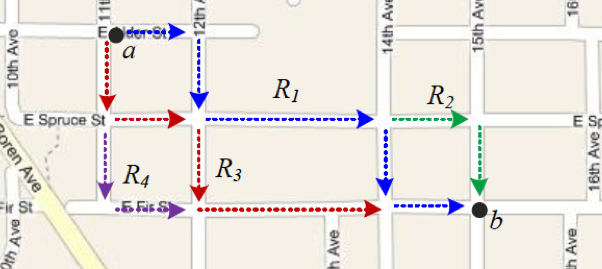
\includegraphics{low_sample_rate}
\centering
\caption{Example of low sampling rate problem}
\end{figure}

The taxi is known to have traversed from point $a$ to point $b$. But there are four possible trajectories from $a$ to $b$. The exact route cannot be determined without additional information in this case.
\subsubsection{Limited GPS accuracy}
After decades of development, the GPS service has achieved great accuracy, but it is still not completely error-free. A report\cite{FP15} in 2015 showed that GPS-enabled smartphones typically have an accuracy of 5 metres \emph{under open sky}. But in a metropolis like Beijing, the actual accuracy may be lower than this value due to the reflection of signals amongst high buildings. Moreover, the data set used in this project was collected in 2009 when GPS devices had lower accuracy than that of today's.

The limited accuracy in GPS devices makes the exact mapping from a GPS data point to a street impossible. In Beijing, there is usually a side road running in parallel with a main road. Due to that limited accuracy, the taxi might be \emph{actually} on the side road but the GPS data point is shown on the main road, or vice versa. 

\section{Related work}
The incentive for carrying out this project comes from a similar project\cite{TDR10}, and similar procedures are followed in this project but with some modifications. 



\chapter{Preliminary Data Processing}
\section{Data Collection and Cleaning}
The taxi GPS data used in this project is collected from the Computational Sensing Lab\cite{BPLL13} at Tsinghua University, Beijing, China. The data set contains approximately 83 million time-stamped taxi GPS records collected from 8,602 taxis in Beijing, from 1 May 2009 to 30 May 2009. The original data set consists of seven fields as shown in Table~\ref{Ta:orig_field}. Longitude and latitude in the data set are defined in the WGS-84\footnote{World Geodetic System} standard coordinate system, which is the reference coordinate system used by the GPS.

\begin{table}
\centering
\begin{tabular}{ | l | l | l | }
\hline
\textbf{Field} & \textbf{Explanation} \\ \hline
CUID & ID for each taxi \\ \hline
UNIX\_EPOCH & Unix timestamp in milliseconds since 1 January 1970\\ \hline
GPS\_LONG & Longitude encoded in WGS-84 multiplied by $10^{5}$\\ \hline
GPS\_LAT & Latitude encoded in WGS-84 multiplied by $10^{5}$ \\ \hline
HEAD & Heading direction in degrees with 0 denoting North\\ \hline
SPEED & Instantaneous speed in metres/second (m/s)\\ \hline
OCCUPIED & Binary indicator of whether the taxi is hired (1) or not (0)\\ \hline
\end{tabular}
\caption{Fields in the original data set}\label{Ta:orig_field}
\end{table}

The original data set came in a binary file format. After the data set was decoded and imported into a MySQL database, the first step in data cleaning was \textbf{to delete all records with zero value in the SPEED field}, since when a taxi is stationary it yields no valuable information about the \emph{trajectory} it is moving along. While being stationary could be due to a traffic jam, this kind of information is well captured by the time difference between the last \emph{non-stationary} data point and the next \emph{non-stationary} data point. 

In addition, all records must have a \emph{unique} pair of CUID and UNIX\_EPOCH fields, since it is not possible for a taxi to appear in two different locations at the same moment in time. This kind of error is likely due to some errors in aggregating the original data set.

\section{Reverse Geocoding}
After the data set was cleaned, the next step was to map each GPS data point to a road segment, which is also known as \emph{reverse geocoding}. A number of algorithms\cite{MAP09} have been proposed for this purpose, but most of them require an additional GIS\footnote{Geographic Information System} database of the road network in Beijing. This project adopted an alternative strategy which leveraged on the existing public APIs\footnote{Application Programming Interface} for reverse geocoding. 

Currently, a number of online mapping platforms provide reverse geocoding services as part of their developer APIs. Amongst others, Google Maps and Baidu Maps offer relatively stable and fast reverse geocoding services. However, due to the ``China GPS shift problem''\cite{GSHF17} where coordinates encoded in WGS-84 format are required by regulations to be shifted by a large and variable amount when displayed on a street map, Google Maps is not able to display a GPS data point correctly because it only supports WGS-84 formats. Figure~\ref{Fig:gps_shift} illustrates the effect of such shift, with the correct location displayed on the right. 

\begin{figure}[h]
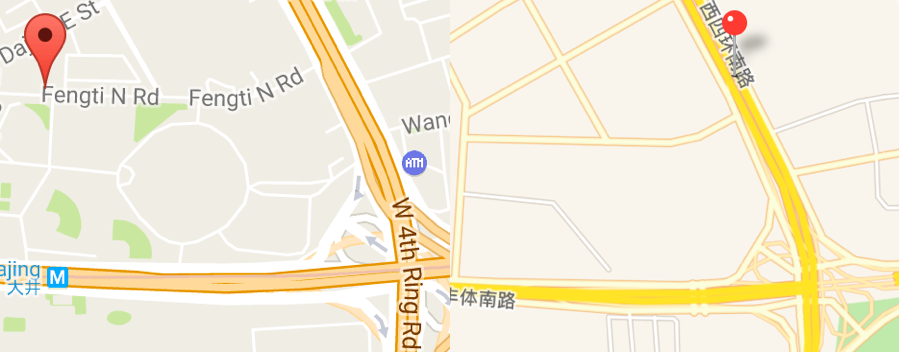
\includegraphics{gps_shift}
\centering
\caption{China GPS shift problem}\label{Fig:gps_shift}
\end{figure}

Baidu Maps, on the other hand, has been using their own coordinate system, BD-09, which is an improved version of the Chinese official coordinate system, GCJ-02. Baidu provides a set of APIs to convert WGS-84 coordinates into BD-09 ones. Therefore, to reverse-geocode the data points, the coordinates must be converted to BD-09 format. To store the converted coordinates as well as the street names obtained from reverse geocoding, four new fields were added to the original data set as shown in Table~\ref{Ta:addtional_field}.

\begin{table}
\centering
\begin{tabular}{ | l | l | l | }
\hline
\textbf{Field} & \textbf{Explanation} \\ \hline
DataUnitID & Nominal primary key for each record \\ \hline
UTC & UNIX\_EPOCH in human readable format \\ \hline
BD09\_LONG & Longitude encoded in BD-09 format\\ \hline
BD09\_LAT & Latitude encoded in BD-09 format\\ \hline
STREET & Street name\\ \hline
\end{tabular}
\caption{Additional fields added to data set}\label{Ta:addtional_field}
\end{table}

In order to use Baidu APIs for coordinate conversion, the following system architecture was set up as shown in Figure~\ref{Fig:basic_architecture}. The Apache HTTP server hides the MySQL database and sends HTTP POST request to Baidu Maps Web API to get converted coordinates. Then it updates the database through PHP \emph{mysqli} utilitity. 

\begin{figure}[h]
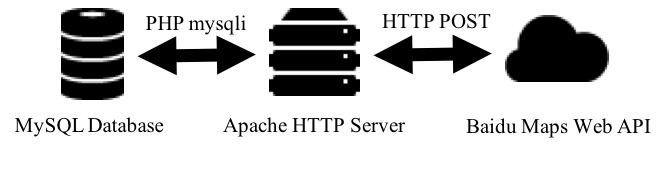
\includegraphics{basic_architecture}
\centering
\caption{Basic system architecture}\label{Fig:basic_architecture}
\end{figure}

After the coordinates were converted from WGS-84 format to BD-09 format, Baidu Maps Web API was used to reverse geocode all GPS data points. However, the system architecture was slightly changed, to accommodate the change in technology used. For reverse geocoding, AJAX\footnote{Asynchronous JavaScript and XML} was used to communicate with the Baidu Maps Web API for speed and unlimited number of requests per day. Therefore, one additional layer was added to the existing system architecture as shown in Figure~\ref{Fig:ajax_architecture}. 

\begin{figure}[h]
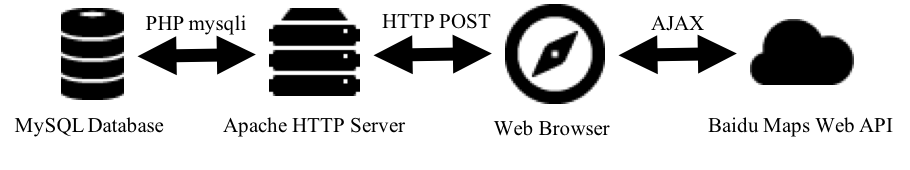
\includegraphics{ajax_architecture}
\centering
\caption{Augmented system architecture}\label{Fig:ajax_architecture}
\end{figure}

Executed in a web browser environment, AJAX sent HTTP POST requests to the Apache HTTP server to fetch the converted coordinates in BD-09 format which were subsequently sent to the Baidu Maps Web API server \emph{asynchronously} via HTTP GET requests. Once the server responded with the name of the road segment, AJAX updated the database by sending another HTTP POST request to the Apache HTTP server. The asynchronous nature of this architecture, however, caused a few problems which are addressed in Section~\ref{outlier_detecting}. 

\section{Outlier Detection}\label{outlier_detecting}
\subsection{Motivation for Outlier Detection}
The Baidu Maps Web API for reverse geocoding is stable and fast, but does not produce no errors. Sometimes, a GPS data point may be mapped to a main road but actually it is on the side road, which is one of the limitations mentioned in Section~\ref{Sec:limitation} or it is actually mapped to a street that Baidu Maps does not recognise. In neither case will Baidu Maps produce a correct reverse geocoding. Moreover, the reverse geocoding process is asynchronous, which means that it is being performed in the background in parallel with the main application thread. Therefore, it is inevitable that some street names may get lost when the records are being updated or a record is updated with a wrong street name. Figure~\ref{Fig:exmp_outlier} shows a drastic example.

\begin{figure}[h]
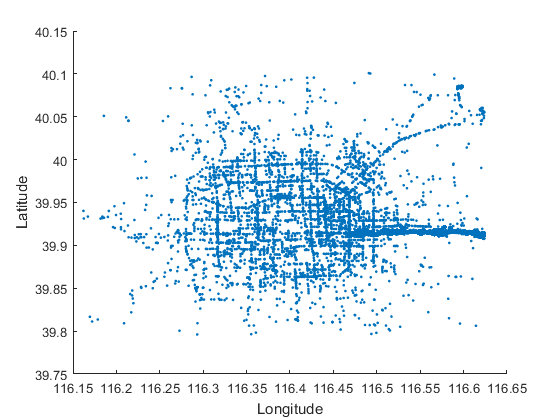
\includegraphics{long_lat_plot}
\centering
\caption{Example of outliers}\label{Fig:exmp_outlier}
\end{figure}

In this example, the Baidu Maps believes that all data points plotted belong to a particular street. But when plotted on a 2-D plane, these data points almost represent the \emph{entire} road network in Beijing. The actual, correct street is represented in the figure as the \emph{thickest} line on the right half of the figure with a longitude ranging from 116.45\textdegree~to 116.65\textdegree.~Erroneous records like those not on the thickest line are known as \emph{outliers} and must be properly identified and removed. This project proposes a novel outlier detection approach based on unsupervised learning whose principle behind is based on Theorem~\ref{Theorem: majority_clustering}.

\begin{defn}[\emph{Reasonable reverse geocoder}]\label{Def:reasonable_geocoder}
A reasonable reverse geocoder always gives its best matching from a GPS data point to a street whenever possible and has an accuracy more than 50\%.
\end{defn}

\begin{theorem}[\emph{Majority Clustering Theorem}]\label{Theorem: majority_clustering}
If a \emph{reasonable reverse geocoder} is used to reverse geocode a set of GPS data points which are mapped to a particular street \emph{in reality}, then, when plotted on a 2-D plane, majority (more than 50\%) of the points must be clustered together to form a rough shape that is similar to the shape of the street that they are supposed to be mapped to. 
\end{theorem}

\begin{proof}
Proof by contradiction. Assume, for the purpose of contradiction, majority (more than 50\%) of the data points that are \emph{indeed} located on the same street are scattered arbitrarily on a 2-D plane after being reverse-geocoded by a reasonable reverse geocoder. In particular, when plotted on a 2-D plane, majority of them do not form a similar shape to that of the street they are supposed to be mapped to. Then, the majority must have been erroneously mapped to some other streets because no single street covers the whole city area. Thus, the reasonable reverse geocoder has only achieved an accuracy less 50\%, which contradicts the Definition~\ref{Def:reasonable_geocoder} of a reasonable reverse geocoder. 
\end{proof}

\subsection{Outlier Identification}\label{SubSec:outlier_identify}
Apparently, Baidu Maps provides a reasonable reverse geocoder because it is of industrial-grade quality and has an accuracy larger than 50\%. Therefore, if a set of points belong to a particular street, after reverse-geocoded by Baidu Maps, majority of them should be clustered to assume a rough shape of that street according to Theorem~\ref{Theorem: majority_clustering}. Based on that, an unsupervised learning technique --- clustering can be used to separate the correctly mapped data points from outliers. 

Many clustering techniques are available\cite{LO05}. Since each record can be represented graphically by a point on a 2-D plane with longitute as the $x$ axis and latitude as the $y$ axis, a \textbf{self-organising feature map}\cite{TK82}(SOFM) seems to be an appropriate technique to use. 

\begin{figure}[h]
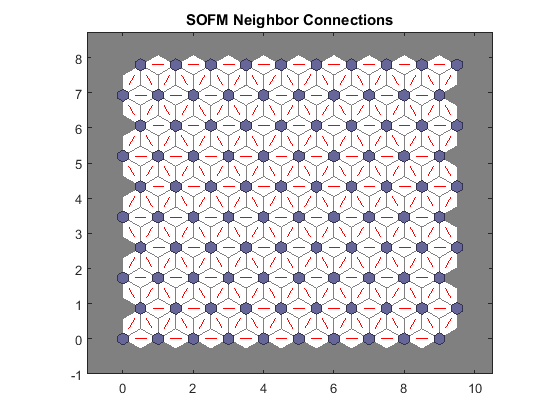
\includegraphics{neighbour_connections}
\centering
\caption{An example of SOFM}\label{Fig:neighbour_connections}
\end{figure}

A self-organising feature map is a form of artificial neural network. It consists of a pre-defined number of interconnected neurons distributed over a 2-D plane as shown in Figure~\ref{Fig:neighbour_connections}. Prior to training, the neurons are randomly scattered among the data points and gradually move to the centroids of the data clusters they represent as they learn the \emph{features} of the training data. Upon termination of the training, all data points near to a particular neuron, in terms of Euclidean distance\footnote{Other distance measures are also possible.}, are assigned to the cluster that neuron represents. Figure~\ref{Fig:sofm_weights} shows the results after the clustering is completed. 

\begin{figure}[h]
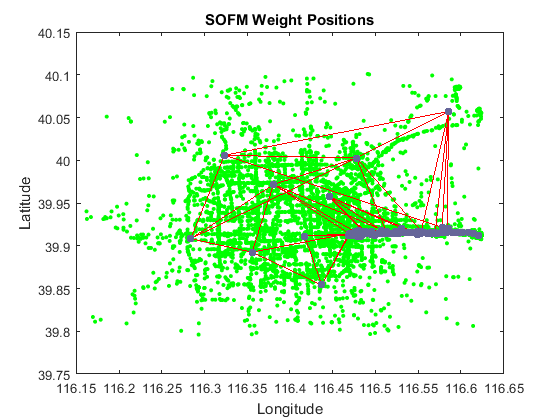
\includegraphics{sofm_weights}
\centering
\caption{Neuron positions after training}\label{Fig:sofm_weights}
\end{figure}

It is clear from the figure that while some neurons represent the clusters of outliers, majority of the neurons are clustered to \emph{cover} the correct street they should represent. A $10\times10$ SOFM was used in this project, so there were at most 100 neurons or equivalently, 100 clusters. Each cluster had a different size. To ensure a thorough removal of the outliers, \textbf{only the top 50\% largest clusters were considered as clusters of correct data points which are called ``legal clusters''. All other clusters were deemed as clusters of outliers}. 

\subsection{Outlier Removal}\label{Subsec:outlier_removal}
Once the legal clusters were identified, a distance threshold was set to remove outliers so that \textbf{whenever the minimum distance between a data point and all centroids of the legal clusters was above the threshold, that data point would be considered as an outlier and removed}. The python-like pseudocode in Listing~\ref{List:code_outlier} describes this idea with more clarity.

%\begin{minipage}{\linewidth}
\begin{lstlisting}[language = Python, caption = {Pseudocode for outlier detection}, label = {List:code_outlier} ,frame=single, numbers=left,stepnumber=1]
for record in records:
	min_distance = math.inf // infinity
	for centroid in centroids:
		min_distance = min(min_distance, \
			get_distance(record, centroid))
	if min_distance > threshold:
		remove(records, record)
\end{lstlisting}
%\end{minipage}

However, the \emph{distance} between a data point and a centroid is not as straightforward as Euclidean distance. A centroid, to some extent, can be imagined as a \emph{real} point on the Earth's surface. To calculate the distance between a data point and a centroid is to calculate the spherical distance which is given by the haversine formula in Theorem~\ref{Theorem: haversine}. 

\begin{theorem}[\emph{Haversine Formula}]\label{Theorem: haversine}
Given two points $P(\lambda_1,\varphi_1)$ and $Q(\lambda_2,\varphi_2)$ on the surface of a sphere, where $\lambda$ and $\varphi$ represent longitude and latitude in radians, their spherical distance (the distance along a great circle of the sphere) is given by\cite{FI06}
\begin{equation}
d = 2R\arcsin{\sqrt{\sin^2\frac{\varphi_2 - \varphi_1}{2} + \cos\varphi_1\cos\varphi_2\sin^2\frac{\lambda_2 - \lambda_1}{2}}} 
\end{equation}
where $R$ is the radius of the sphere. 
\end{theorem}

Since the Earth is not a perfect sphere, $R$ varies with latitude. Theorem~\ref{Theorem: radius_latitide} suggests how to calculate the Earth radius at any latitude. 

\begin{theorem}[\emph{Radius at any Latitude}]\label{Theorem: radius_latitide}
Given a latitude $\varphi$ in radians, a polar radius $R_{p}$ and an equatorial radius $R_{e}$, the spheroid's radius at that latitude is given by\cite{EAR17}
\begin{equation}
R(\varphi) = \sqrt{\frac{(R_{e}^2\cos\varphi)^2 + (R_{p}^2\sin\varphi)^2}{(R_{e}\cos\varphi)^2 + (R_{p}\sin\varphi)^2}}
\end{equation}
\end{theorem}

It is known that $R_{e} = 6,378,137$ metres and $R_{p} = 6,356,752$ metres on the Earth\cite{NASA16} and that Beijing's latitude is about 39\textdegree N. Therefore, the distance between a data point and a centroid can be calculated. For this project, two thresholds were selected: 30 metres and 50 metres. The thresholds were set in a way that it ensured there was sufficient data for subsequent machine learning tasks while the estimates were as least affected as possible by outliers. If the threshold were set to a too small value, the remaining data could not have been sufficient; on the other hand, however, if the threshold were set to a too big value, the accuracy of the final results would have been subject to outliers. 

\begin{figure}[h]
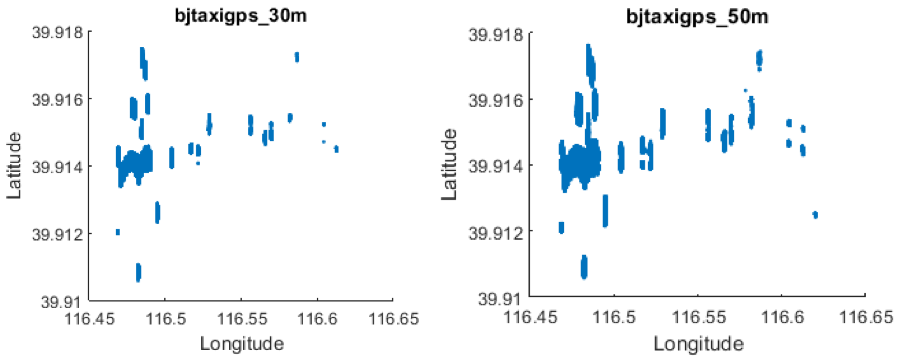
\includegraphics{30m_50m}
\centering
\caption{Plot of data points after outlier removal}\label{Fig:after_removal}
\end{figure}

After the outliers were removed, two data sets remained. They are hereinafter referred to as \emph{bjtaxigps\_30m}, where outliers were filtered by a threshold of 30 metres and \emph{bjtaxigps\_50m}, where outliers were filtered by a threshold of 50 metres, respectively. bjtaxigps\_30m contains approximately 51 million records while bjtaxigps\_50m has 59 million. All algorithms described hereinafter are applicable to both data sets. Figure~\ref{Fig:after_removal} gives a plot of the data points from both data sets. Clearly, the data points are now contained in a much smaller area and roughly form a shape similar to that of the street they are mapped to. 
\chapter{Landmark Graph Construction}
\begin{defn}[\emph{Landmark}]\label{Def:ldmk}
A landmark is a road segment that is frequently traversed by taxi drivers according to the taxi GPS trajectory database. \cite{TDR10}
\end{defn}
The concept of a landmark is proposed primarily for two reasons. First, as mentioned in the Section~\ref{Sec:limitation}, the taxi GPS trajectories do not necessarily cover every road segment in a city's road network and the low-sampling-rate problem makes determining the exact route on which a taxi traversed difficult. Therefore, it is not possible to estimate the time cost for each road segment. However, ignoring the length of a road segment and considering it as an abstract ``landmark'' make estimating the travel time between two \emph{landmarks} viable. 

Moreover, the notion of landmarks closely follows the way how drivers remember the driving routes in daily life\cite{TDR10}. For instance, a driving route could be described as ``go straight on the 4th Avenue, turn right at the 7th Street and exit at the Smith Road''. Drivers tend to use familiar road segments as landmarks to guide their directions.

This chapter describes the procedures for constructing a landmark graph in order to estimate the time cost between two landmarks. But before that, the taxi GPS trajectories must be separated into a set of \emph{trips}.

\section{Trip Identification}
\begin{defn}[\emph{Trip}]\label{Def:trip}
A trip is a set of chronologically ordered GPS records belonging to one taxi that satisfies either condition:
\begin{enumerate}
\item A passenger is on the taxi, namely, all records in the set have an OCCUPIED field of value 1 or, 
\item No passenger is on the taxi, but the time difference between \emph{any} two consecutive records is no larger than 3 minutes.
\end{enumerate}
\end{defn}

Table~\ref{Ta:trip_identification} gives a tiny example of trip identification.

\begin{table}[h]
\centering
\resizebox{\columnwidth}{!}{
\begin{tabular}{ | l | l | l | l | l | l | l | l | l | l | l | l | l | }
\hline
\textbf{CUID} & \textbf{UTC} & \textbf{GPS\_LONG} & \textbf{GPS\_LAT} & \textbf{OCCUPIED} & \textbf{TRIP\_ID} \\\hline
1	&	1/5/2009 0:02:00	&	116.39616	&	39.81294	&	0	&	4552265\\ \hline
1	&	1/5/2009 0:04:00	&	116.39575	&	39.82296	&	0	&	4552265\\ \hline
1	&	1/5/2009 0:07:00	&	116.39567	&	39.82774	&	0	&	4552265\\ \hline
1	&	1/5/2009 17:08:00	&	116.30142	&	39.98105	&	1	&	1\\ \hline
1	&	1/5/2009 17:10:00	&	116.29514	&	39.98419	&	1	&	1\\ \hline
1	&	1/5/2009 17:11:00	&	116.28959	&	39.98289	&	1	&	1\\ \hline
1	&	1/5/2009 17:12:00	&	116.28087	&	39.97552	&	1	&	1\\ \hline
1	&	1/5/2009 17:16:00	&	116.26813	&	39.93537	&	1	&	1\\ \hline
1	&	1/5/2009 18:11:00	&	116.36537	&	39.95019	&	0	&	4552271\\ \hline
1	&	1/5/2009 18:12:00	&	116.36546	&	39.94886	&	0	&	4552271\\ \hline
1	&	1/5/2009 18:13:00	&	116.35927	&	39.94528	&	0	&	4552271\\ \hline
\end{tabular}}
\caption{An example of trip identification}\label{Ta:trip_identification}
\end{table}

Clearly, all records in Table~\ref{Ta:trip_identification} belong to one taxi (taxi with CUID = 1) and are sorted chronologically. The first three records, although no passengers are aboard, are considered to be in the same \emph{trip} because the time difference between any two consecutive records is no larger than 3 minute. The next five records constitute another trip, even though the last two records have a time difference of 4 minutes, since a passenger is on the taxi (OCCIPIED = 1). Following the same reasoning as the first three's, the last three records are treated as one trip. Listing~\ref{List:code_trip} gives the pseudocode for trip identification.

\begin{lstlisting}[language = Python, caption = {Pseudocode for trip identification}, label = {List:code_trip} ,frame=single, numbers=left,stepnumber=1]
curr_tripid = 1
last_occup = curr_occup = records[0].OCCUPIED
last_unixepoch = curr_unixepoch = records[0].UNIX_EPOCH
for recd in records:
	curr_occup = recd.OCCUPIED
	curr_unixepoch = recd.UNIX_EPOCH
	if curr_occup != last_occup:
		++curr_tripid
	elif (curr_occup == 0) && \
		(curr_unixepoch - last_unixepoch > threshold):
			++curr_tripid
	recd.TRIP_ID = curr_tripid
	last_occup = curr_occup
	last_unixepoch = curr_unixepoch
\end{lstlisting}

It is noteworthy that although the middle five records with OCCUPIED = 1 come chronologically after the first three records, they are nevertheless assigned a smaller TRIP\_ID. This is due to an adjustment made to the actual implementation of the algorithm. The \emph{actual} algorithm operates in two stages. It first identifies trips for all records with OCCUPIED = 1; only in the second stage does it identify trips for records with OCCUPIED = 0. The rationale for this arrangement is to give priority to the records with passengers aboard, because \textbf{these records are guaranteed to belong to one trip}. In fact, the second condition for identifying trips in Definition~\ref{Def:trip} is more of a heuristic rather than a theorem. It is meant to provide sufficient data for subsequent machine learning tasks with reasonable accuracy.

\section{Landmark Counting}
Definition~\ref{Def:trip} states that whether recognising a particular road segment as a landmark or not is based on some notions of frequency. Only if a road segment is visited by drivers frequently enough is it recognised as a landmark. In this project, the notion of frequency is given by Definition~\ref{Def:frequency}.

\begin{defn}[\emph{Frequency of a Road Segment}]\label{Def:frequency}
The frequency of a road segment is the sum of \emph{unique} occurrences of that road segment in each trip. 
\end{defn}

Table~\ref{Ta:frequency_count} illustrates how the frequency of a road segment is calculated. In Trip 4552265, Street A occurs twice but \textbf{its frequency increases only by one}. Similarly, Street C occur three times and Street A occur twice in Trip 1, but \textbf{their occurrences only add one to their frequencies}. Therefore, even though Street B \emph{appears} less times than Street A or Street C, \textbf{all streets have the same frequency of 2}, based on this set of records.  
\begin{table}[h]
\centering
\resizebox{\columnwidth}{!}{
\begin{tabular}{ | l | l | l | l | l | l | l | l | l | l | l | l | l | }
\hline
\textbf{CUID} & \textbf{UTC} & \textbf{GPS\_LONG} & \textbf{GPS\_LAT} & \textbf{Street} & \textbf{TRIP\_ID} \\\hline
1	&	1/5/2009 0:02:00	&	116.39616	&	39.81294	&	A	&	4552265\\ \hline
1	&	1/5/2009 0:04:00	&	116.39575	&	39.82296	&	A	&	4552265\\ \hline
1	&	1/5/2009 0:07:00	&	116.39567	&	39.82774	&	B	&	4552265\\ \hline
1	&	1/5/2009 17:08:00	&	116.30142	&	39.98105	&	C	&	1\\ \hline
1	&	1/5/2009 17:10:00	&	116.29514	&	39.98419	&	C	&	1\\ \hline
1	&	1/5/2009 17:11:00	&	116.28959	&	39.98289	&	C	&	1\\ \hline
1	&	1/5/2009 17:12:00	&	116.28087	&	39.97552	&	A	&	1\\ \hline
1	&	1/5/2009 17:16:00	&	116.26813	&	39.93537	&	A	&	1\\ \hline
1	&	1/5/2009 18:11:00	&	116.36537	&	39.95019	&	B	&	4552271\\ \hline
1	&	1/5/2009 18:12:00	&	116.36546	&	39.94886	&	C	&	4552271\\ \hline
1	&	1/5/2009 18:13:00	&	116.35927	&	39.94528	&	C	&	4552271\\ \hline
\end{tabular}}
\caption{An illustration of frequency counting}\label{Ta:frequency_count}
\end{table}

Currently, a number of online mapping platforms provide reverse geocoding services as part of their developer APIs. Amongst others, Google Maps and Baidu Maps offer relatively stable and fast reverse geocoding services. However, due to the ``China GPS shift problem''\cite{GSHF17} where coordinates encoded in WGS-84 format are required by regulations to be shifted by a large and variable amount when displayed on a street map, Google Maps is not able to display a GPS data point correctly because it only supports WGS-84 formats. Figure~\ref{Fig:gps_shift} illustrates the effect of such shift, with the correct location displayed on the right. 

\begin{figure}[h]
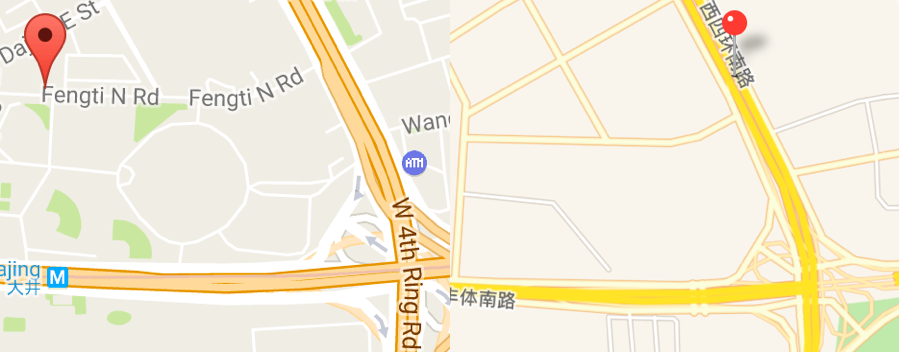
\includegraphics{gps_shift}
\centering
\caption{China GPS shift problem}\label{Fig:gps_shift}
\end{figure}

Baidu Maps, on the other hand, has been using their own coordinate system, BD-09, which is an improved version of the Chinese official coordinate system, GCJ-02. Baidu provides a set of APIs to convert WGS-84 coordinates into BD-09 ones. Therefore, to reverse-geocode the data points, the coordinates must be converted to BD-09 format. To store the converted coordinates as well as the street names obtained from reverse geocoding, four new fields were added to the original data set as shown in Table~\ref{Ta:addtional_field}.

\begin{table}
\centering
\begin{tabular}{ | l | l | l | }
\hline
\textbf{Field} & \textbf{Explanation} \\ \hline
DataUnitID & Nominal primary key for each record \\ \hline
BD09\_LONG & Longitude encoded in BD-09 format\\ \hline
BD09\_LAT & Latitude encoded in BD-09 format\\ \hline
STREET & Street name\\ \hline
\end{tabular}
\caption{Additional fields added to data set}\label{Ta:addtional_field}
\end{table}

In order to use Baidu APIs for coordinate conversion, the following system architecture was set up as shown in Figure~\ref{Fig:basic_architecture}. The Apache HTTP server hides the MySQL database and sends HTTP POST request to Baidu Maps Web API to get converted coordinates. Then it updates the database through PHP \emph{mysqli} utilitity. 

\begin{figure}[h]
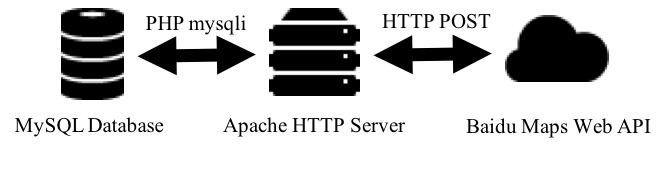
\includegraphics{basic_architecture}
\centering
\caption{Basic system architecture}\label{Fig:basic_architecture}
\end{figure}

After the coordinates were converted from WGS-84 format to BD-09 format, Baidu Maps Web API was used to reverse geocode all GPS data points. However, the system architecture was slightly changed, to accommodate the change in technology used. For reverse geocoding, AJAX\footnote{Asynchronous JavaScript and XML} was used to communicate with the Baidu Maps Web API for speed and unlimited number of requests per day. Therefore, one additional layer was added to the existing system architecture as shown in Figure~\ref{Fig:ajax_architecture}. 

\begin{figure}[h]
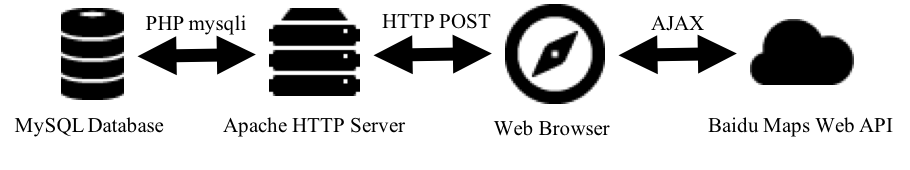
\includegraphics{ajax_architecture}
\centering
\caption{Augmented system architecture}\label{Fig:ajax_architecture}
\end{figure}

Executed in a web browser environment, AJAX sent HTTP POST requests to the Apache HTTP server to fetch the converted coordinates in BD-09 format which were subsequently sent to the Baidu Maps Web API server \emph{asynchronously} via HTTP GET requests. Once the server responded with the name of the road segment, AJAX updated the database by sending another HTTP POST request to the Apache HTTP server. The asynchronous nature of this architecture, however, caused a few problems which are addressed in Section~\ref{outlier_detecting}. 

\section{Outlier Detection}\label{outlier_detecting}
\subsection{Motivation for Outlier Detection}
The Baidu Maps Web API for reverse geocoding is stable and fast, but does not produce no errors. Sometimes, a GPS data point may be mapped to a main road but actually it is on the side road, which is one of the limitations mentioned in Section~\ref{Sec:limitation} or it is actually mapped to a street that Baidu Maps does not recognise. In neither case will Baidu Maps produce a correct reverse geocoding. Moreover, the reverse geocoding process is asynchronous, which means that it is being performed in the background in parallel with the main application thread. Therefore, it is inevitable that some street names may get lost when the records are being updated or a record is updated with a wrong street name. Figure~\ref{Fig:exmp_outlier} shows a drastic example.

\begin{figure}[h]
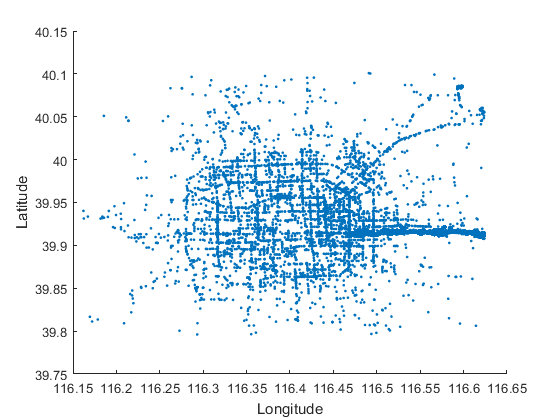
\includegraphics{long_lat_plot}
\centering
\caption{Example of outliers}\label{Fig:exmp_outlier}
\end{figure}

In this example, the Baidu Maps believes that all data points plotted belong to a particular street. But when plotted on a 2-D plane, these data points almost represent the \emph{entire} road network in Beijing. The actual, correct street is represented in the figure as the \emph{thickest} line on the right half of the figure with a longitude ranging from 116.45\textdegree~to 116.65\textdegree.~Erroneous records like those not on the thickest line are known as \emph{outliers} and must be properly identified and removed. This project proposes a novel outlier detection approach based on unsupervised learning whose principle behind is based on Theorem~\ref{Theorem: majority_clustering}.

\begin{defn}[\emph{Reasonable reverse geocoder}]\label{Def:reasonable_geocoder}
A reasonable reverse geocoder always gives its best matching from a GPS data point to a street whenever possible and has an accuracy more than 50\%.
\end{defn}

\begin{theorem}[\emph{Majority Clustering Theorem}]\label{Theorem: majority_clustering}
If a \emph{reasonable reverse geocoder} is used to reverse geocode a set of GPS data points which are mapped to a particular street \emph{in reality}, then, when plotted on a 2-D plane, majority (more than 50\%) of the points must be clustered together to form a rough shape that is similar to the shape of the street that they are supposed to be mapped to. 
\end{theorem}

\begin{proof}
Proof by contradiction. Assume, for the purpose of contradiction, majority (more than 50\%) of the data points that are \emph{indeed} located on the same street are scattered arbitrarily on a 2-D plane after being reverse-geocoded by a reasonable reverse geocoder. In particular, when plotted on a 2-D plane, majority of them do not form a similar shape to that of the street they are supposed to be mapped to. Then, the majority must have been erroneously mapped to some other streets because no single street covers the whole city area. Thus, the reasonable reverse geocoder has only achieved an accuracy less 50\%, which contradicts the Definition~\ref{Def:reasonable_geocoder} of a reasonable reverse geocoder. 
\end{proof}

\subsection{Outlier Identification}
Apparently, Baidu Maps provides a reasonable reverse geocoder because it is of industrial-grade quality and has an accuracy larger than 50\%. Therefore, if a set of points belong to a particular street, after reverse-geocoded by Baidu Maps, majority of them should be clustered to assume a rough shape of that street according to Theorem~\ref{Theorem: majority_clustering}. Based on that, an unsupervised learning technique --- clustering can be used to separate the correctly mapped data points from outliers. 

Many clustering techniques are available\cite{LO05}. Since each record can be represented graphically by a point on a 2-D plane with longitute as the $x$ axis and latitude as the $y$ axis, a \textbf{self-organising feature map}\cite{TK82}(SOFM) seems to be an appropriate technique to use. 

\begin{figure}[h]
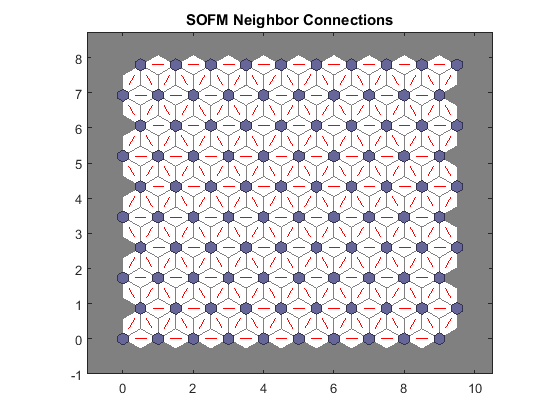
\includegraphics{neighbour_connections}
\centering
\caption{An example of SOFM}\label{Fig:neighbour_connections}
\end{figure}

A self-organising feature map is a form of artificial neural network. It consists of a pre-defined number of interconnected neurons distributed over a 2-D plane as shown in Figure~\ref{Fig:neighbour_connections}. Prior to training, the neurons are randomly scattered among the data points and gradually move to the centroids of the data clusters they represent as they learn the \emph{features} of the training data. Upon termination of the training, all data points near to a particular neuron, in terms of Euclidean distance\footnote{Other distance measures are also possible.}, are assigned to the cluster that neuron represents. Figure~\ref{Fig:sofm_weights} shows the results after the clustering is completed. 

\begin{figure}[h]
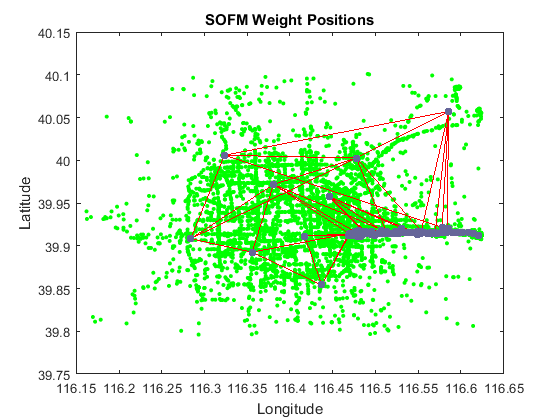
\includegraphics{sofm_weights}
\centering
\caption{Neuron positions after training}\label{Fig:sofm_weights}
\end{figure}

It is clear from the figure that while some neurons represent the clusters of outliers, majority of the neurons are clustered to \emph{cover} the correct street they should represent. A $10\times10$ SOFM was used in this project, so there were at most 100 neurons or equivalently, 100 clusters. Each cluster had a different size. To ensure a thorough removal of the outliers, \textbf{only the top 50\% largest clusters were considered as clusters of correct data points which are called ``legal clusters''. All other clusters were deemed as clusters of outliers}. 

\subsection{Outlier Removal}
Once the legal clusters were identified, a distance threshold was set to remove outliers so that \textbf{whenever the minimum distance between a data point and all centroids of the legal clusters was above the threshold, that data point would be considered as an outlier and removed}. The python-like pseudocode in Listing~\ref{List:code_outlier} describes this idea with more clarity.

%\begin{minipage}{\linewidth}
\begin{lstlisting}[language = Python, caption = {Pseudocode for outlier detection}, label = {List:code_outlier} ,frame=single, numbers=left,stepnumber=1]
for record in records:
	min_distance = math.inf // infinity
	for centroid in centroids:
		min_distance = min(min_distance, \
			get_distance(record, centroid))
	if min_distance > threshold:
		remove(records, record)
\end{lstlisting}
%\end{minipage}

However, the \emph{distance} between a data point and a centroid is not as straightforward as Euclidean distance. A centroid, to some extent, can be imagined as a \emph{real} point on the Earth's surface. To calculate the distance between a data point and a centroid is to calculate the spherical distance which is given by the haversine formula in Theorem~\ref{Theorem: haversine}. 

\begin{theorem}[\emph{Haversine Formula}]\label{Theorem: haversine}
Given two points $P(\lambda_1,\varphi_1)$ and $Q(\lambda_2,\varphi_2)$ on the surface of a sphere, where $\lambda$ and $\varphi$ represent longitude and latitude in radians, their spherical distance (the distance along a great circle of the sphere) is given by\cite{FI06}
\begin{equation}
d = 2R\arcsin{\sqrt{\sin^2\frac{\varphi_2 - \varphi_1}{2} + \cos\varphi_1\cos\varphi_2\sin^2\frac{\lambda_2 - \lambda_1}{2}}} 
\end{equation}
where $R$ is the radius of the sphere. 
\end{theorem}

Since the Earth is not a perfect sphere, $R$ varies with latitude. Theorem~\ref{Theorem: radius_latitide} suggests how to calculate the Earth radius at any latitude. 

\begin{theorem}[\emph{Radius at any Latitude}]\label{Theorem: radius_latitide}
Given a latitude $\varphi$ in radians, a polar radius $R_{p}$ and an equatorial radius $R_{e}$, the spheroid's radius at that latitude is given by\cite{EAR17}
\begin{equation}
R(\varphi) = \sqrt{\frac{(R_{e}^2\cos\varphi)^2 + (R_{p}^2\sin\varphi)^2}{(R_{e}\cos\varphi)^2 + (R_{p}\sin\varphi)^2}}
\end{equation}
\end{theorem}

It is known that $R_{e} = 6,378,137$ metres and $R_{p} = 6,356,752$ metres on the Earth\cite{NASA16} and that Beijing's latitude is about 39\textdegree N. Therefore, the distance between a data point and a centroid can be calculated. For this project, two thresholds were selected: 30 metres and 50 metres. The thresholds were set in a way that it ensured there was sufficient data for subsequent machine learning tasks while the estimates were as least affected as possible by outliers. If the threshold were set to a too small value, the remaining data could not have been sufficient; on the other hand, however, if the threshold were set to a too big value, the accuracy of the final results would have been subject to outliers. 

\begin{figure}[h]
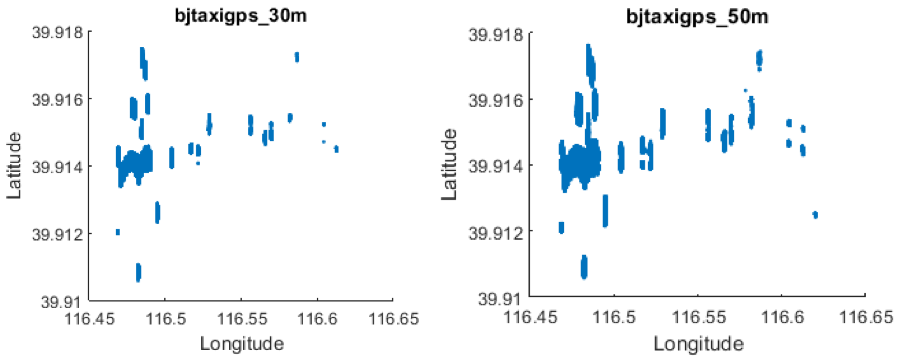
\includegraphics{30m_50m}
\centering
\caption{Plot of data points after outlier removal}\label{Fig:after_removal}
\end{figure}

After the outliers were removed, two data sets remained. They are hereinafter referred to as \emph{bjtaxigps\_30m}, where outliers were filtered by a threshold of 30 metres and \emph{bjtaxigps\_50m}, where outliers were filtered by a threshold of 50 metres, respectively. bjtaxigps\_30m contains approximately 51 million records while bjtaxigps\_50m has 59 million. All algorithms described hereinafter are applicable to both data sets. Figure~\ref{Fig:after_removal} gives a plot of the data points from both data sets. Clearly, the data points are now contained in a much smaller area and roughly form a shape similar to that of the street they are mapped to. 
\chapter{Time-dependent Edge Cost Estimation}\label{Chap:4}
Chapter~\ref{Ch:ldmk_graph} describes the general procedures for constructing a landmark graph. To find a time-dependent shortest route on a landmark graph, the time-dependent edge cost must be calculated. In this project, the time-dependent edge cost specifically refers to travel time, but in theory, it can refer to any quantity that can be described as a time-dependent edge cost function of the form $w : E,t \rightarrow \mathbb{R}$. In practice, it sometimes also refers to fuel consumptions or taxi fares. This chapter introduces a machine learning-based approach to estimate the travel time of each \emph{significant edge} in a landmark graph at a particular moment in time. 

\begin{defn}[\emph{Support}]
A support for an edge $e$ in a landmark graph $G=(V,E)$ is the number of times that $e$ appears. 
\end{defn}

\begin{defn}[\emph{Significant Edge}]
A significant edge in a landmark graph $G=(V,E)$ is an edge $e \in E$ that has a support at least $m$, where $m$ is a parameter specified in advance.
\end{defn}

The purpose of defining significant edges is to eliminate those edges that are seldom traversed by taxi drivers, as estimating the travel time of those edges will not be very accurate. The parameter $m$ also represents a level of \emph{confidence}, that is, to what extent it is true that this edge \emph{really} exists in the real world. 

Everyday experiences show that the travel time of a particular road usually has different time-varying patterns in weekdays as compared to that in weekends or public holidays. For instance, it is likely that, on weekdays, the travel time of a particular road has one \emph{peak} at 8 a.m. when people travel to work and the other peak at 6 p.m. when people return home after work. But when it is weekends or public holidays, the travel time of that road may have a peak at 10 a.m. when people go for holiday activities with families and the other peak at only about 8 p.m. when the whole day's celebrations are over. 

Based on this intuition, two separate landmark graphs were built in this project, with one for weekdays and the other for weekends or public holidays. Moreover, as mentioned in Section~\ref{Subsec:outlier_removal}, 
two data sets, bjtaxigps\_30m and bjtaxigps\_50m, remained after outlier removal based on different thresholds set for removing outliers. Therefore, in total, \emph{four} landmark graphs were built in this project and they are summarised in Table~\ref{Ta:ldmkgraphs}, although their names are self-explanatory. 

\begin{table}[h!]
\centering
\resizebox{\columnwidth}{!}{
\begin{tabular}{ | c | c | }
\hline
\textbf{Landmark Graph} & \textbf{Data Source} \\ \hline
wrkd\_ldmkgraph\_30m & weekday trajectories in bjtaxigps\_30m\\\hline
holi\_ldmkgraph\_30m & holiday trajectories in bjtaxigps\_30m \\\hline
wrkd\_ldmkgraph\_50m & weekday trajectories in bjtaxigps\_50m\\\hline
holi\_ldmkgraph\_50m  & holiday trajectories in bjtaxigps\_50m\\ \hline
\end{tabular}}
\caption{An summary of landmark graphs}\label{Ta:ldmkgraphs}
\end{table}

\section{Travel Time Distribution}
\begin{figure}[h!]
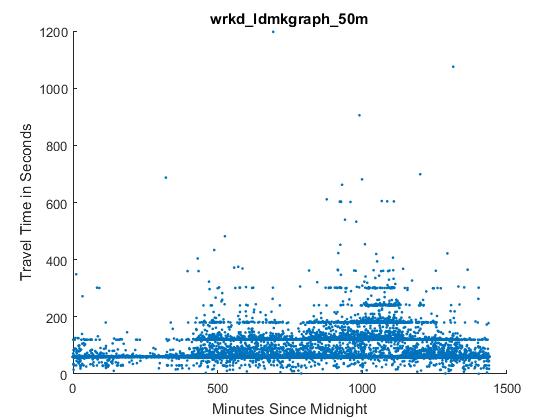
\includegraphics[scale=0.85]{trvltime_scatter}
\centering
\caption{An example of travel time patterns}\label{Fig:wrkd_50m_trvltime}
\end{figure}

Figure~\ref{Fig:wrkd_50m_trvltime} illustrates a scatter plot of the travel time of a particular landmark graph edge during the course of a weekday. It can be observed that the travel time does not seem to be a single-valued function with respect to time of the day, as one may expect; rather, the scatter points tend to gather around some values and form some \emph{clusters}. For instance, when it is 500 minutes since midnight, namely 8:20~a.m., the travel time seems to have three main clusters which are represented by three horizontal lines formed by the scatter points. When it is 1,000 minutes since midnight, namely 4:40~p.m., there are about five such lines. This pattern is attributable to three possible reasons:
\begin{enumerate}
\item Drivers may actually choose different routes to travel between the two landmarks, which cannot be captured by the landmark graph since it only knows a driver has traversed between the two landmarks but not the exact route. Different routes have different traffic conditions and speed limitations, therefore the travel time varies;
\item Drivers have different driving skills, preferences and behaviours. Some drivers just drive faster than others, even if the road conditions are similar and;
\item The GPS devices on taxis reported locations \emph{periodically}, therefore, durations like 60 seconds or 120 seconds are very commonly seen in the landmark graphs. Even if the \emph{actual} travel time is 53 seconds, it is still recorded as 60 seconds. This corresponds to the low-sampling-rate problem mentioned in Section~\ref{Sec:limitation}. 
\end{enumerate}

\begin{figure}[h!]
\centering
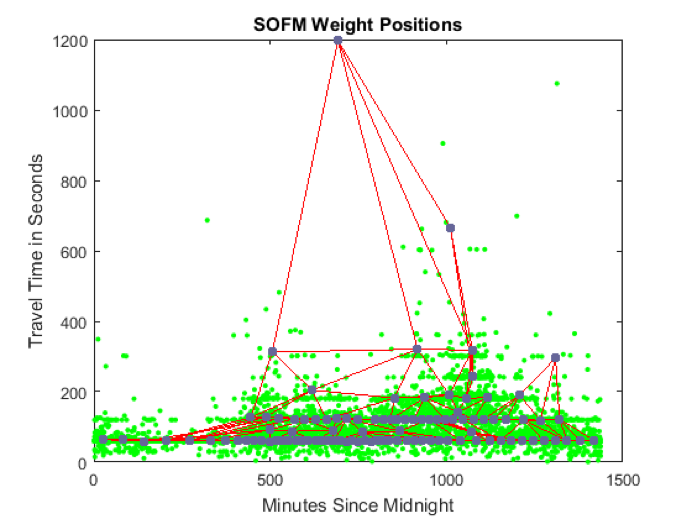
\includegraphics[scale=0.85]{trvltime_clus} 
\caption{Final positions of the neurons}\label{Fig:trvltime_clus}
\end{figure}

Therefore, it is not possible to fit the scatter points with a single-valued function. Rather, the clustering technique should first be employed to identify the travel time clusters. Like in Section~\ref{SubSec:outlier_identify}, a \textbf{self-organising feature map} is used to cluster the scatter points. Figure~\ref{Fig:trvltime_clus} shows the final positions of the neurons at the end of the training.

\begin{figure}[h!]
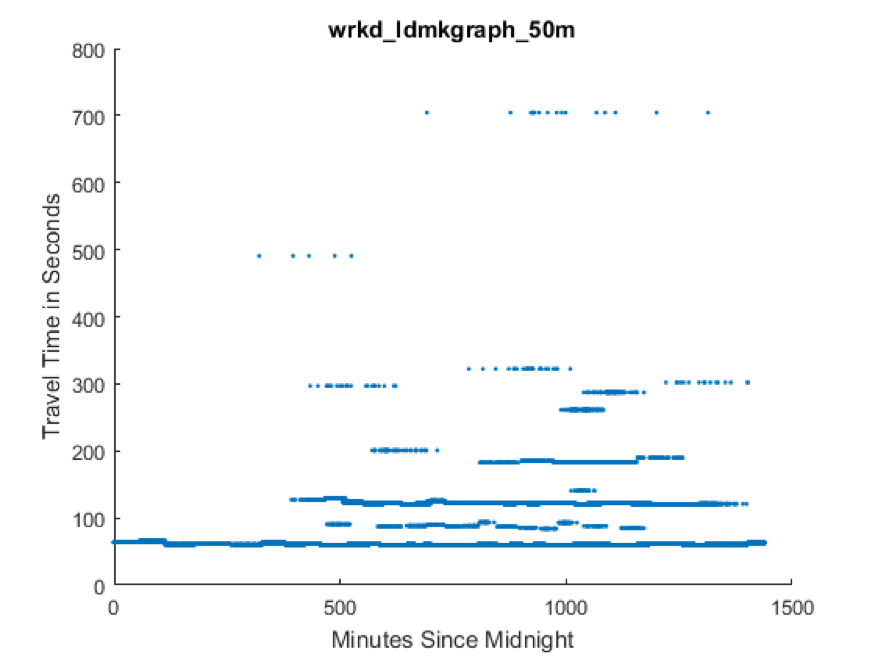
\includegraphics[scale=0.85]{trvltime_neurons}
\centering
\caption{An example of representing data points with centroids}\label{Fig:trvltime_neurons}
\end{figure}

One merit of SOFM clustering is \emph{feature extraction}. In this case, after the training is completed, the SOFM has learned some features about the travel time at different time of the day and expressed its understanding by moving its neurons to the centroids of the clusters. Now, \textbf{the data points can be represented by their respective centroids}. Figure~\ref{Fig:trvltime_neurons} shows the effect of replacing each data point's value with their centroids'. The clusters are clearly shown by the horizontal lines formed by those centroids. 

Representing data points with cluster centroids or features learned provides the benefit of \emph{generalisation}. The data set used in this project, albeit large in size, is nevertheless a small \emph{sample} of the \emph{population} of taxi trajectories over time. In other words, these trajectory records are only the \emph{observed} ones but there are potentially infinite number of trajectories that cannot be all observed. The only information known about them is that \textbf{they must fit into one of the clusters} after undergoing the same procedures described in the previous chapters. The use of centroids instead of real data points also takes into consideration the unobserved trajectories and reflects the real underlying patterns. In fact, generalisation is an advantage that all neural network-based methods share. 

\begin{figure}[h!]
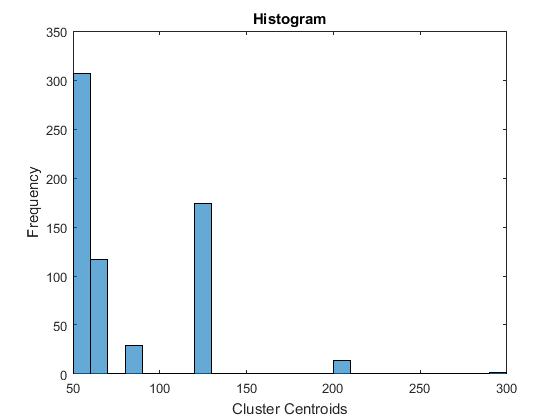
\includegraphics[scale=0.85]{clus_histo}
\centering
\caption{An example of distribution of clusters}\label{Fig:clus_histo}
\end{figure}

Now that the clusters are identified, Figure~\ref{Fig:clus_histo} shows a histogram of clusters within the 10:00~a.m. to 10:30~a.m. interval. It can be observed that within a particular time interval, there are many clusters of travel time and each cluster has different sizes. To describe the travel time pattern within a particular time interval, the histogram is converted into a cumulative probability distribution of clusters which is then fitted with Weibull Distribution described in Theorem~\ref{Theorem: weibull_dist}. 

\begin{theorem}[\emph{Weibull Distribution}]\label{Theorem: weibull_dist}
A Weibull Distribution is described by two strictly positive parameters, the scale parameter $\alpha$ and the shape parameter $\beta$, and has a \textbf{probability distribution function} of \cite{WEDI}
\begin{equation}
f(x | \alpha, \beta) = \frac{\beta}{\alpha}\cdot(\frac{x}{\alpha})^{\beta - 1}\cdot e^{-(x / \alpha)^{\beta}}.
\end{equation}
Correspondingly, its \textbf{cumulative distribution function} is given by \cite{WEIB}
\begin{equation}
F(x | \alpha, \beta) = \int_{0}^{x} f(t | \alpha, \beta) dt = 1 - e^{-(x / \alpha)^{\beta}}.
\end{equation}
\end{theorem}

\begin{figure}[h!]
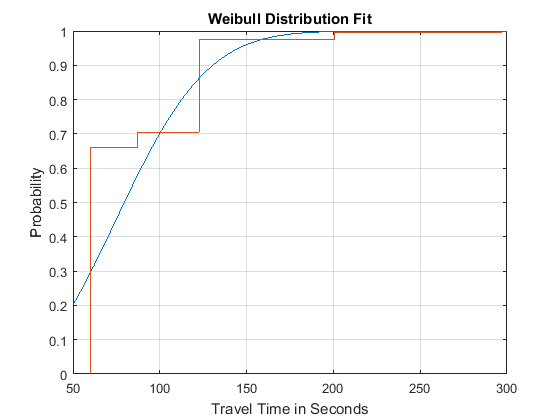
\includegraphics[scale=0.85]{weibull_fit}
\centering
\caption{Weibull Distribution Fit}\label{Fig:weibull_fit}
\end{figure}

Figure~\ref{Fig:weibull_fit} shows an example of fitting a cumulative probability distribution with Weibull Distribution. The red line represents the cumulative probability distribution and the blue line indicates the best Weibull Distribution fit estimated by maximum likelihood. 

In the referencing paper \cite{TDR10}, it uses inverse Gaussian distribution to fit the centroid distribution. However, as some experiments showed, inverse Gaussian distribution does not always work, especially when the centroids actually have a uniform distribution, namely, when only one cluster appears in the time interval. In that case, Weibull distribution will have the shape parameter $\beta = \infty$ but it still can give the correct result. 

The cumulative distribution function of Weibull distribution is good at calculating the probability whereby the travel time $t$ is less than a particular value. For instance, the probability of the travel time for this landmark graph edge being less than or equal to 100 seconds is approximately $P(t\leq100) = 0.7$ according to the Weibull distribution curve in Figure~\ref{Fig:weibull_fit}. But to estimate the travel time of a landmark graph edge is in fact the \emph{reverse}: given a known probability $P$, find the corresponding travel time $t$, which is exactly the inverse Weibull cumulative distribution function does. 

\begin{theorem}[\emph{Inverse Weibull Cumulative Distribution Function}]\label{Theorem: weibull_inverse_dist}
The inverse Weibull cumulative distribution function is defined as
\begin{equation}
F^{-1}(x | \alpha, \beta) = G(p) = \alpha(-ln(1 - p)) ^ {1/\beta}
\end{equation}
where $p$ is the given probability.
\end{theorem}

In practice, the probability $p$ corresponds to some subjective measures of a driver's driving skill. It represents how fast a driver drives as compared to other drivers. If a driver has a $p$ value of 0.2, it means that this driver usually drives faster than 80\% ($1 - 0.2$) drivers. This concept is formally defined in Definition~\ref{Def:opti_index}.

\begin{defn}[\emph{Optimism Index}]\label{Def:opti_index}
A optimism index $p$ indicates how optimistic a driver feels about his or her driving skills \cite{TDR10}. A driver with an optimism index of $p_{0}$ usually drives faster than $(1 - p_{0})\%$ drivers. 
\end{defn}

The optimism index of a driver can be set by the driver in advance, although it may be subject to illusory superiority\footnote{In a 1986 experiment, \emph{80\%} participants rated their driving skills \emph{above-average} \cite{IFD86}.}. It can also be set to the mean value by default or learned from the driver's trajectory history. 

With optimism index defined, it is easy to estimate the travel time using Theorem~\ref{Theorem: weibull_inverse_dist}. However, it is worth mentioning that for a cumulative probability distribution function $F(x)$, the probability of a single value is zero, namely, $F(x_{0}) = 0$; only a range of values can have positive probabilities. Therefore, the travel time calculated from optimism index should really be a \emph{range} of travel time. For instance, if the optimism index is $p = 0.7$, the correct result should be $t \leq 100$ based on Figure~\ref{Fig:weibull_fit}, which means that for a driver with an optimism index of 0.7, his or her travel time is \emph{at most} 100 seconds. No exact value can be determined. However, in the context of this project, only the \emph{worst-case} travel time is considered; therefore, the driver is said to have an expected travel time of 100 seconds. 

\section{Travel Time Evaluation}
After the travel time distributions for each significant edge were determined, an eva\-luation was conducted to ascertain the accuracy of the travel time estimates. In this project, the estimates made by Theorem~\ref{Theorem: weibull_inverse_dist} were compared against real-time estimates made by Baidu Maps at various times of the day. 

Some complications do arise, however, because the two vertices of each significant edge are actually two \emph{landmarks}. Definition~\ref{Def:ldmk} states that a landmark is essentially a road segment with its length ignored. But in estimating the travel time between two landmarks, the length of the landmarks cannot be ignored and has profound effects on how the travel time should be calculated. 

\begin{figure}[h!]
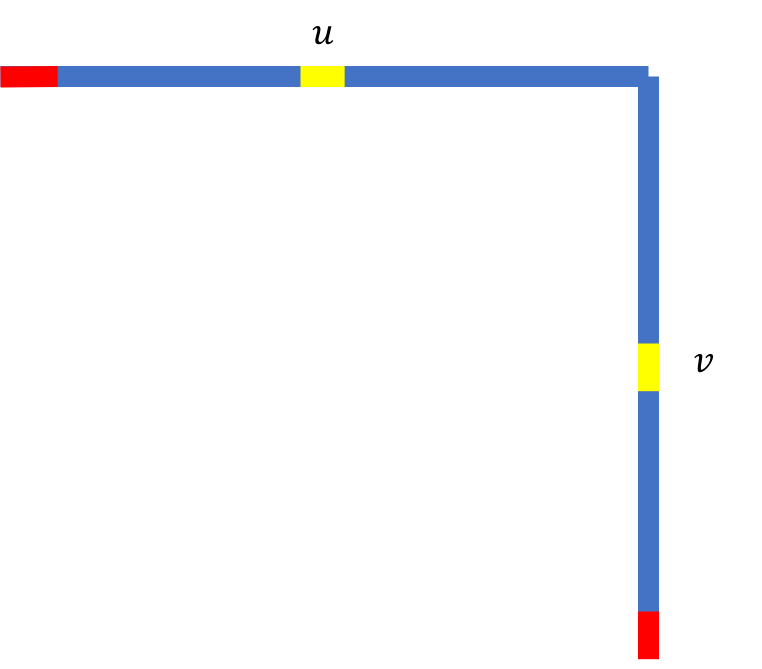
\includegraphics[scale=0.8]{ldmk_travel}
\centering
\caption{An example of different landmark travel time}\label{Fig:ldmk_travel}
\end{figure}

Imagine there are two landmarks $u$ and $v$, respectively, and each has a length of $L$ as shown in Figure~\ref{Fig:ldmk_travel}. Then, there are potentially infinite number of ways of `traveling from $u$ to $v$', because the starting point could be any points on $u$ and the ending point could be any points on $v$. If a driver starts at the red point on $u$ and stops at the red point on $v$, the total distance is $2L$ and the total time is $T$. But had the driver stopped at the yellow mid-point on $v$, the total distance would be $1.5L$ and the total time would be $3T/4$, assuming the speed is constant. 

Therefore, it is difficult to give a \emph{definite} estimate of the travel time between two landmarks. In this project, the \textbf{median travel time} is instead used to represent the travel time between two landmarks. It describes the \emph{typical} travel time a driver should expect. An example of a median case is that the diver starts at the yellow mid-point on $u$ and ends at the yellow mid-point on $v$. But there are in fact infinite number of median cases. 

The most significant 150 edges were selected to be evaluated, from \emph{each} of the four landmark graphs listed in Table~\ref{Ta:ldmkgraphs}. For each edge $(u, v)$, 20\% of the trajectories with $u$ as starting point and $v$ as ending point were randomly sampled. These trajectories represent some random trips between $u$ and $v$ with varying distances. Baidu Maps API was then used to estimate the travel time for each trajectory in real time, after which the median of all the estimates was selected as Baidu's estimate for the travel time between $u$ and $v$. Finally, Theorem~\ref{Theorem: weibull_inverse_dist} was used to calculate its own the travel time estimate which was then compared against Baidu's. Table~\ref{Ta:eval_res} summarises the evaluation results for all 150 significant edges. 

\begin{table}[h!]
\centering
\resizebox{\columnwidth}{!}{
\begin{tabular}{ | c | c | c | c |}
\hline
\textbf{Landmark Graph} & \textbf{RMSE} & \textbf{Mean Error Ratio} & \textbf{Mean No. of Samples Per Edge} \\ \hline
wrkd\_ldmkgraph\_50m & 78.84 & -0.009 & 1824.60 \\ \hline
wrkd\_ldmkgraph\_30m & 87.96 & -0.065 & 1507.56 \\ \hline
holi\_ldmkgraph\_50m & 87.39 & -0.16 & 832.96 \\ \hline
holi\_ldmkgraph\_30m & 76.41 & -0.14 & 681.89 \\ \hline
\end{tabular}}
\caption{Summary of Evaluation Results}\label{Ta:eval_res}
\end{table}

Assuming a Baidu's estimate is $b_{i}$ and the corresponding project's estimate is $\hat{b}_{i}$, then the Root Mean Square Error (RMSE) is given by:
\begin{equation}
RMSE = \sqrt{\frac{\sum_{i = 1}^{N}(\hat{b}_{i} - b_{i})^{2}}{N}}
\end{equation}
where $N$ is the total number of estimates; and the Mean Error Ratio (MER) is given by:
\begin{equation}
MER = \frac{1}{N}\sum_{i = 1}^{N}\frac{\hat{b}_{i} - b_{i}}{b_{i}}
\end{equation}

The RMSE gives an overall measure of accuracy. For instance, the RMSE for landmark graph \emph{wrkd\_ldmkgraph\_50m} turned out to be 78.58, which means that on average, the difference between Baidu's estimates and Theorem~\ref{Theorem: weibull_inverse_dist}'s estimate was 78.58 seconds. But whether this difference is significant or not depends on the scale of Baidu's estimates. For a Baidu's estimate of 30 seconds, 78.58 seconds may be considered significant, but for an estimate of 200 seconds, it may be acceptable. 

Therefore, MER is designed to take into account the scale of Baidu's estimates. It computes the ratio between the error and Baidu's estimate. A positive MER indicates that on average Theorem~\ref{Theorem: weibull_inverse_dist} tends to have larger estimates than Baidu's; on the other hand, a negative MER indicates that on average, Theorem~\ref{Theorem: weibull_inverse_dist} tends to have smaller estimates than Baidu's. 

Another technique to gauge Theorem~\ref{Theorem: weibull_inverse_dist}'s performance is linear regression. An ordered pair of estimates $(b_{i}, \hat{b}_{i})$ can be treated as a point in a 2-D Cartesian system. In the \emph{ideal} case, $\hat{b}_{i}$ should be equal to $b_{i}$, therefore, all points should form a straight line with a slope of 1 and an intercept of 0 when plotted. In the general cases, the regression equation gives the relationship between $b_{i}$ and $\hat{b}_{i}$. If the slope of the regression equation is less than 1, then $\hat{b}_{i}$ is expected to be less than $b_{i}$ in \emph{most} cases depending on the intercept. Figure~\ref{Fig:regression_plot} shows the regression plots. 

In summary, the estimates Theorem~\ref{Theorem: weibull_inverse_dist} gave were smaller than Baidu's estimates in most cases, which to some extent, was actually expected. The data set was collected in 2009 but Baidu Maps was giving \emph{real-time} estimates. Eight years since then, the travel time in the entire road network should have increased in general, due to increase in car ownership. Nevertheless, it still provides reasonable estimates with RMSE around 90 seconds. 

\begin{figure}[h!]
\begin{subfigure}{.5\textwidth}
\centering
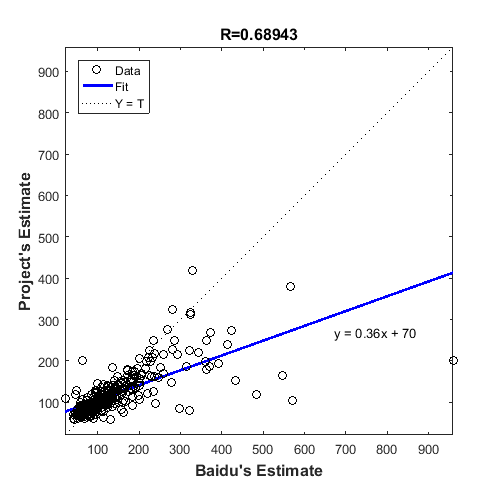
\includegraphics[width = .9\linewidth]{wrkd_50m_reg}
\caption{wrkd\_ldmkgraph\_50m}
\label{Fig:wrkd_50m_reg}
\end{subfigure}
\begin{subfigure}{.5\textwidth}
\centering
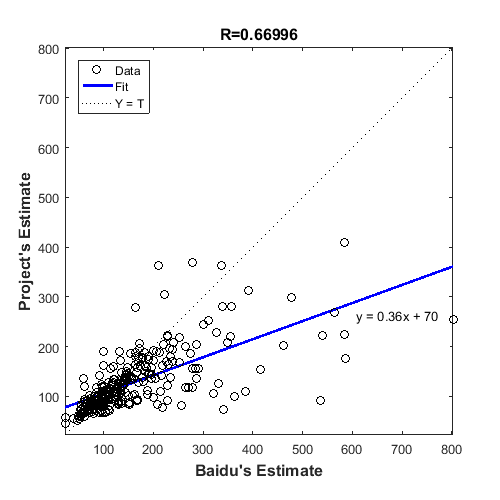
\includegraphics[width = .9\linewidth]{wrkd_30m_reg}
\caption{wrkd\_ldmkgraph\_30m}
\label{Fig:wrkd_30m_reg}
\end{subfigure}

\begin{subfigure}{.5\textwidth}
\centering
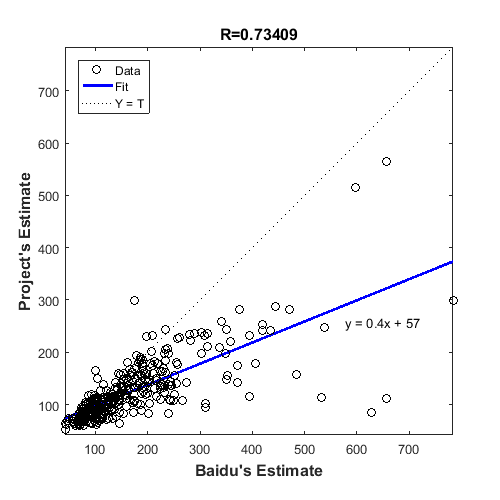
\includegraphics[width = .9\linewidth]{holi_50m_reg}
\caption{holi\_ldmkgraph\_50m}
\label{Fig:holi_50m_reg}
\end{subfigure}
\begin{subfigure}{.5\textwidth}
\centering
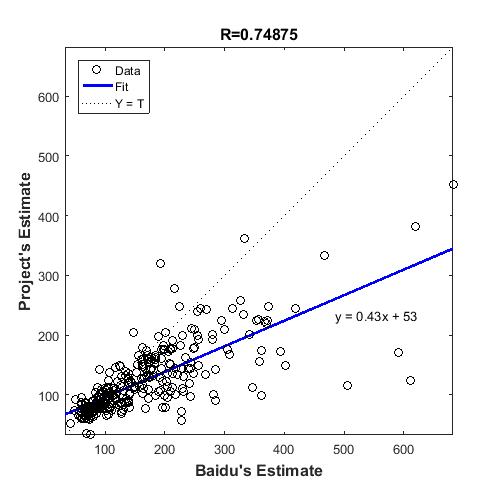
\includegraphics[width = .9\linewidth]{holi_30m_reg}
\caption{holi\_ldmkgraph\_30m}
\label{Fig:holi_30m_reg}
\end{subfigure}

\caption{Regression Plots}
\label{Fig:regression_plot}
\end{figure}

\section{Shortest Path Calculation}
\begin{defn}[\emph{FIFO Graph}]\label{Def:fifo_graph}
A time-dependent graph $G=(V,E)$ with a dynamic weight function $w : E,t \rightarrow \mathbb{R}$ is a FIFO graph \cite{TDS08} iff for every edge $(u, v) \in E$
\begin{equation}
w(u, v, t_{0}) \leq \Delta t + w(u, v, t_{0} + \Delta t), \forall \Delta t \geq 0
\end{equation}
\end{defn}

Once the time-varying patterns of edge costs are determined, calculating a shortest path in a landmark graph is straightforward, provided the landmark graph is a FIFO graph\footnote{If the graph is not a FIFO graph, the problem is NP-hard if waiting is not allowed at any vertices} as defined in Definition~\ref{Def:fifo_graph}. 

An equivalent way of expressing FIFO property is that, if a person leaves vertex $u$ at time $t_{0}$, then any persons who leave vertex $u$ at a later time $t_{0} + \Delta t$ will not be able to reach vertex $v$ earlier than the first person. In practice, transport networks are said to have FIFO property \cite{TDR10}, therefore, a landmark graph can be considered as a FIFO graph. Then the Dijkstra's shortest path algorithm can be applied directly but with a modification that the edge costs are computed dynamically as the algorithm proceeds. Figure~\ref{Fig:dynamic_update} shows an example of dynamically updating edge costs. 

\begin{figure}[h!]
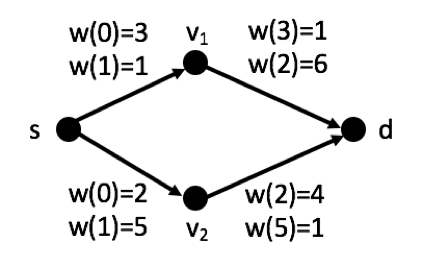
\includegraphics[scale=1]{shortest_path_demo}
\centering
\caption{An example of updating edge costs dynamically}\label{Fig:dynamic_update}
\end{figure}

If a taxi leaves $s$ at time $t = 0$, the edge $(s, v_{1})$ and $(s, v_{2})$ will have a time-dependent travel time of 3 and 2, respectively. If the taxi follows the current fastest edge $(s, v_{2})$, when it arrives at $v_{2}$ the time-dependent travel time of the edge $(v_{2}, d)$ at time $t = 2$ will be 4, giving a total travel time 6. But should the taxi follow the edge $(s, v_{1})$, the time-dependent travel time of the edge $(v_{1}, d)$ at $t = 3$ would be 1, giving a total travel time of 4. Therefore, path $s \leadsto v_{1} \leadsto d$ is the time-dependent shortest path. The same process applies when the taxi leaves $s$ at time $t = 1$, but the time-dependent shortest path will be path $s \leadsto v_{2} \leadsto d$. This example is also a FIFO graph: path $s \leadsto v_{1} \leadsto d$ would still be the shortest path, should another taxi \emph{wait} at $s$ until $t = 1$. Listing~\ref{List:code_dijkstra} gives the pseudocode for the modified Dijkstra's Algorithm. 

\begin{lstlisting}[language = Python, caption = {Pseudocode for Modified Dijkstra's Algorithm}, label = {List:code_dijkstra} ,frame=single, numbers=left,stepnumber=1, mathescape=true, escapeinside={(*}{*)}]
Input: a landmark graph $G=(V, E)$, source $s$ (*and*) destination $d$
Ouput: a predecessor graph $G_{p}=(V_{p}, E_{p})$
// EAT = Earliest Arrival Time
predecessor = dict{s : None}
pq = queue.PriorityQueue()
s.EAT = 0
pq.put(s)
for vertex in $G.V - \{s\}$:
    vertex.EAT = $\infty$
    pq.put(vertex)
while not pq.empty():
    hd = pq.get()
    for v in hd.neighbours:
    	if hd.EAT + $w(s, v, hd.EAT)$ < v.EAT:
	    v.EAT = hd.EAT + $w(s, v, hd.EAT)$
	    predecessor[v] = hd
\end{lstlisting}

Upon termination of the algorithm in Listing~\ref{List:code_dijkstra}, a predecessor graph whose edges are \emph{reversed} shortest paths from $s$ to other vertices are constructed. Listing~\ref{List:code_printpath} provides a recursive method to print out the shortest path from $s$ to $d$. 

\begin{lstlisting}[language = Python, caption = {Pseudocode for Printing Shortest Paths}, label = {List:code_printpath} ,frame=single, numbers=left,stepnumber=1, mathescape=true, escapeinside={(*}{*)}]
Input: a predecessor graph $G_{p}=(V_{p}, E_{p})$ (*and*) a destination $d$
Ouput: a shortest path $s \leadsto d$

def print_path(predecessor, dst):
    pred = predecessor[dst]
    if pred is None:
    	print(dst.name)
    else:
    	print_path(predecessor, pred)
	print('$\rightarrow$' + dst.name)
	
print_path(predecessor, d)
\end{lstlisting}

\chapter{Shortest Path Calculation}


\begin{defn}[\emph{Significant Edge}]
A significant edge in a landmark graph $G=(V,E)$ is an edge $e \in E$ that has a support at least $m$, where $m$ is a parameter specified in advance.
\end{defn}

The purpose of defining significant edges is to eliminate those edges that are seldom traversed by taxi drivers, as estimating the travel time of those edges will not be very accurate. The parameter $m$ also represents a level of \emph{confidence}, that is, to what extent it is true that this edge \emph{really} exists in the real world. 

Everyday experiences show that the travel time of a particular road usually has different time-varying patterns in weekdays as compared to that in weekends or public holidays. For instance, it is likely that, on weekdays, the travel time of a particular road has one \emph{peak} at 8 a.m. when people travel to work and the other peak at 6 p.m. when people return home after work. But when it is weekends or public holidays, the travel time of that road may have a peak at 10 a.m. when people go for holiday activities with families and the other peak at only about 8 p.m. when the whole day's celebrations are over. 

Based on this intuition, two separate landmark graphs were built in this project, with one for weekdays and the other for weekends or public holidays. Moreover, as mentioned in Section~\ref{Subsec:outlier_removal}, 
two data sets, bjtaxigps\_30m and bjtaxigps\_50m, remained after outlier removal based on different thresholds set for removing outliers. Therefore, in total, \emph{four} landmark graphs were built in this project and they are summarised in Table~\ref{Ta:ldmkgraphs}, although their names are self-explanatory. 

\begin{table}[h!]
\centering
\resizebox{\columnwidth}{!}{
\begin{tabular}{ | c | c | }
\hline
\textbf{Landmark Graph} & \textbf{Data Source} \\ \hline
wrkd\_ldmkgraph\_30m & weekday trajectories in bjtaxigps\_30m\\\hline
holi\_ldmkgraph\_30m & holiday trajectories in bjtaxigps\_30m \\\hline
wrkd\_ldmkgraph\_50m & weekday trajectories in bjtaxigps\_50m\\\hline
holi\_ldmkgraph\_50m  & holiday trajectories in bjtaxigps\_50m\\ \hline
\end{tabular}}
\caption{An summary of landmark graphs}\label{Ta:ldmkgraphs}
\end{table}

\section{Travel Time Distribution}
\begin{figure}[h!]
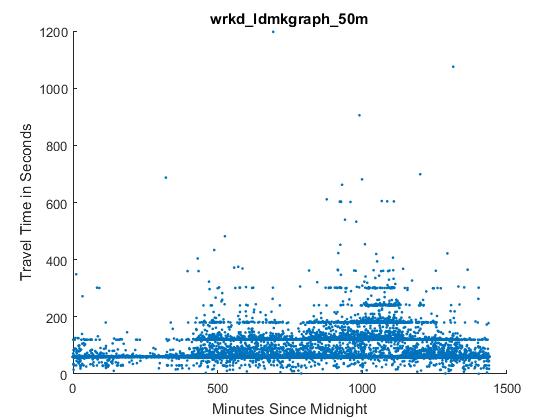
\includegraphics[scale=0.85]{trvltime_scatter}
\centering
\caption{An example of travel time patterns}\label{Fig:wrkd_50m_trvltime}
\end{figure}

Figure~\ref{Fig:wrkd_50m_trvltime} illustrates a scatter plot of the travel time of a particular landmark graph edge during the course of a weekday. It can be observed that the travel time does not seem to be a single-valued function with respect to time of the day, as one may expect; rather, the scatter points tend to gather around some values and form some \emph{clusters}. For instance, when it is 500 minutes since midnight, namely 8:20~a.m., the travel time seems to have three main clusters which are represented by three horizontal lines formed by the scatter points. When it is 1,000 minutes since midnight, namely 4:40~p.m., there are about five such lines. This pattern is attributable to three possible reasons:
\begin{enumerate}
\item Drivers may actually choose different routes to travel between the two landmarks, which cannot be captured by the landmark graph since it only knows a driver has traversed between the two landmarks but not the exact route. Different routes have different traffic conditions and speed limitations, therefore the travel time varies;
\item Drivers have different driving skills, preferences and behaviours. Some drivers just drive faster than others, even if the road conditions are similar and;
\item The GPS devices on taxis reported locations \emph{periodically}, therefore, durations like 60 seconds or 120 seconds are very commonly seen in the landmark graphs. Even if the \emph{actual} travel time is 53 seconds, it is still recorded as 60 seconds. This corresponds to the low-sampling-rate problem mentioned in Section~\ref{Sec:limitation}. 
\end{enumerate}

\begin{figure}[h!]
\centering
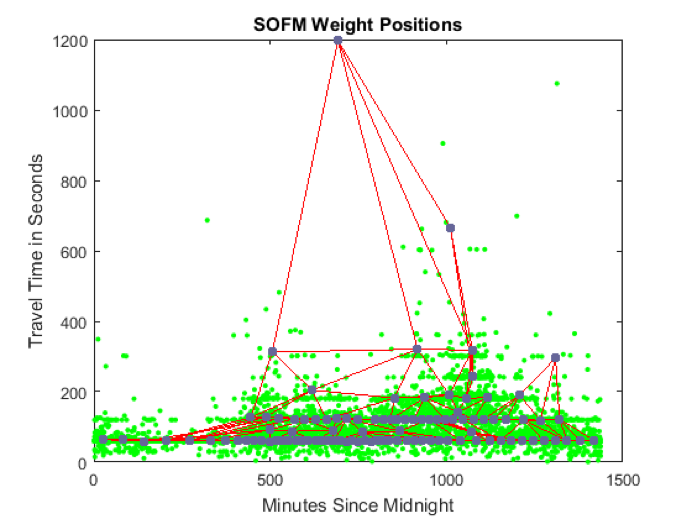
\includegraphics[scale=0.85]{trvltime_clus} 
\caption{Final positions of the neurons}\label{Fig:trvltime_clus}
\end{figure}

Therefore, it is not possible to fit the scatter points with a single-valued function. Rather, the clustering technique should first be employed to identify the travel time clusters. Like in Section~\ref{SubSec:outlier_identify}, a \textbf{self-organising feature map} is used to cluster the scatter points. Figure~\ref{Fig:trvltime_clus} shows the final positions of the neurons at the end of the training.

\begin{figure}[h!]
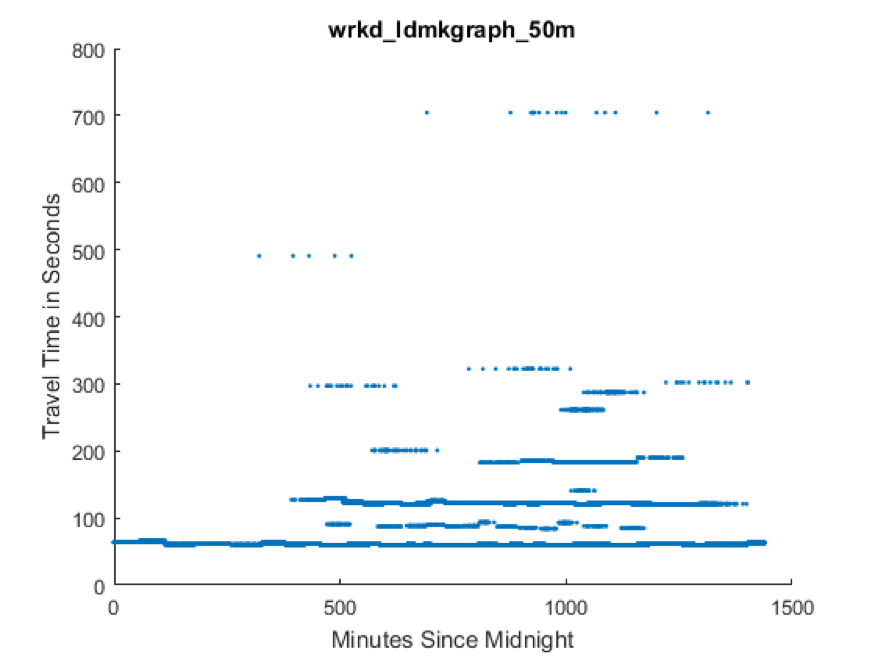
\includegraphics[scale=0.85]{trvltime_neurons}
\centering
\caption{An example of representing data points with centroids}\label{Fig:trvltime_neurons}
\end{figure}

One merit of SOFM clustering is \emph{feature extraction}. In this case, after the training is completed, the SOFM has learned some features about the travel time at different time of the day and expressed its understanding by moving its neurons to the centroids of the clusters. Now, \textbf{the data points can be represented by their respective centroids}. Figure~\ref{Fig:trvltime_neurons} shows the effect of replacing each data point's value with their centroids'. The clusters are clearly shown by the horizontal lines formed by those centroids. 

Representing data points with cluster centroids or features learned provides the benefit of \emph{generalisation}. The data set used in this project, albeit large in size, is nevertheless a small \emph{sample} of the \emph{population} of taxi trajectories over time. In other words, these trajectory records are only the \emph{observed} ones but there are potentially infinite number of trajectories that cannot be all observed. The only information known about them is that \textbf{they must fit into one of the clusters} after undergoing the same procedures described in the previous chapters. The use of centroids instead of real data points also takes into consideration the unobserved trajectories and reflects the real underlying patterns. In fact, generalisation is an advantage that all neural network-based methods share. 

\begin{figure}[h!]
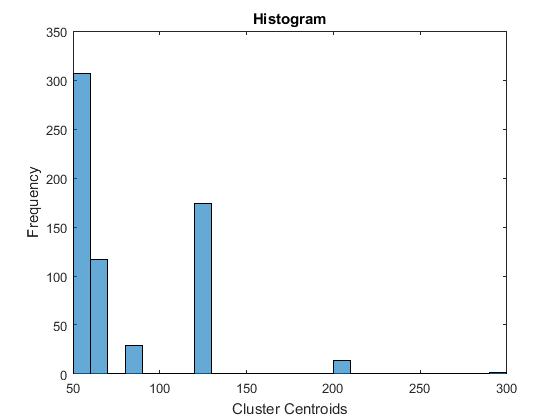
\includegraphics[scale=0.85]{clus_histo}
\centering
\caption{An example of distribution of clusters}\label{Fig:clus_histo}
\end{figure}

Now that the clusters are identified, Figure~\ref{Fig:clus_histo} shows a histogram of clusters within the 10:00~a.m. to 10:30~a.m. interval. It can be observed that within a particular time interval, there are many clusters of travel time and each cluster has different sizes. To describe the travel time pattern within a particular time interval, the histogram is converted into a cumulative probability distribution of clusters which is then fitted with Weibull Distribution described in Theorem~\ref{Theorem: weibull_dist}. 

\begin{theorem}[\emph{Weibull Distribution}]\label{Theorem: weibull_dist}
A Weibull Distribution is described by two strictly positive parameters, the scale parameter $\alpha$ and the shape parameter $\beta$, and has a \textbf{probability distribution function} of \cite{WEDI}
\begin{equation}
f(x | \alpha, \beta) = \frac{\beta}{\alpha}\cdot(\frac{x}{\alpha})^{\beta - 1}\cdot e^{-(x / \alpha)^{\beta}}.
\end{equation}
Correspondingly, its \textbf{cumulative distribution function} is given by \cite{WEIB}
\begin{equation}
F(x | \alpha, \beta) = \int_{0}^{x} f(t | \alpha, \beta) dt = 1 - e^{-(x / \alpha)^{\beta}}.
\end{equation}
\end{theorem}

\begin{figure}[h!]
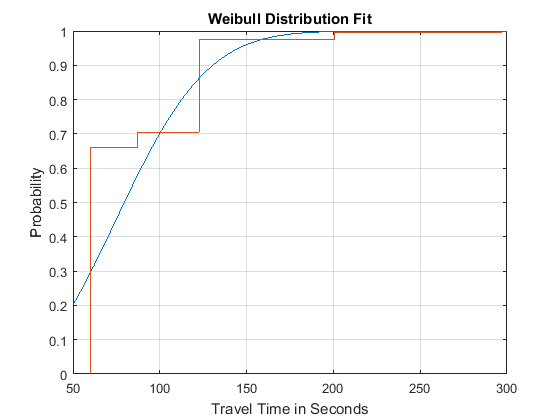
\includegraphics[scale=0.85]{weibull_fit}
\centering
\caption{Weibull Distribution Fit}\label{Fig:weibull_fit}
\end{figure}

Figure~\ref{Fig:weibull_fit} shows an example of fitting a cumulative probability distribution with Weibull Distribution. The red line represents the cumulative probability distribution and the blue line indicates the best Weibull Distribution fit estimated by maximum likelihood. 

In the referencing paper \cite{TDR10}, it uses inverse Gaussian distribution to fit the centroid distribution. However, as some experiments showed, inverse Gaussian distribution does not always work, especially when the centroids actually have a uniform distribution, namely, when only one cluster appears in the time interval. In that case, Weibull distribution will have the shape parameter $\beta = \infty$ but it still can give the correct result. 

The cumulative distribution function of Weibull distribution is good at calculating the probability whereby the travel time $t$ is less than a particular value. For instance, the probability of the travel time for this landmark graph edge being less than or equal to 100 seconds is approximately $P(t\leq100) = 0.7$ according to the Weibull distribution curve in Figure~\ref{Fig:weibull_fit}. But to estimate the travel time of a landmark graph edge is in fact the \emph{reverse}: given a known probability $P$, find the corresponding travel time $t$, which is exactly the inverse Weibull cumulative distribution function does. 

\begin{theorem}[\emph{Inverse Weibull Cumulative Distribution Function}]\label{Theorem: weibull_inverse_dist}
The inverse Weibull cumulative distribution function is defined as
\begin{equation}
F^{-1}(x | \alpha, \beta) = G(p) = \alpha(-ln(1 - p)) ^ {1/\beta}
\end{equation}
where $p$ is the given probability.
\end{theorem}

In practice, the probability $p$ corresponds to some subjective measures of a driver's driving skill. It represents how fast a driver drives as compared to other drivers. If a driver has a $p$ value of 0.2, it means that this driver usually drives faster than 80\% ($1 - 0.2$) drivers. This concept is formally defined in Definition~\ref{Def:opti_index}.

\begin{defn}[\emph{Optimism Index}]\label{Def:opti_index}
A optimism index $p$ indicates how optimistic a driver feels about his or her driving skills \cite{TDR10}. A driver with an optimism index of $p_{0}$ usually drives faster than $(1 - p_{0})\%$ drivers. 
\end{defn}

The optimism index of a driver can be set by the driver in advance, although it may be subject to illusory superiority\footnote{In a 1986 experiment, \emph{80\%} participants rated their driving skills \emph{above-average} \cite{IFD86}.}. It can also be set to the mean value by default or learned from the driver's trajectory history. 

With optimism index defined, it is easy to estimate the travel time using Theorem~\ref{Theorem: weibull_inverse_dist}. However, it is worth mentioning that for a cumulative probability distribution function $F(x)$, the probability of a single value is zero, namely, $F(x_{0}) = 0$; only a range of values can have positive probabilities. Therefore, the travel time calculated from optimism index should really be a \emph{range} of travel time. For instance, if the optimism index is $p = 0.7$, the correct result should be $t \leq 100$ based on Figure~\ref{Fig:weibull_fit}, which means that for a driver with an optimism index of 0.7, his or her travel time is \emph{at most} 100 seconds. No exact value can be determined. However, in the context of this project, only the \emph{worst-case} travel time is considered; therefore, the driver is said to have an expected travel time of 100 seconds. 

\section{Travel Time Evaluation}
After the travel time distributions for each significant edge were determined, an eva\-luation was conducted to ascertain the accuracy of the travel time estimates. In this project, the estimates made by Theorem~\ref{Theorem: weibull_inverse_dist} were compared against real-time estimates made by Baidu Maps at various times of the day. 

Some complications do arise, however, because the two vertices of each significant edge are actually two \emph{landmarks}. Definition~\ref{Def:ldmk} states that a landmark is essentially a road segment with its length ignored. But in estimating the travel time between two landmarks, the length of the landmarks cannot be ignored and has profound effects on how the travel time should be calculated. 

\begin{figure}[h!]
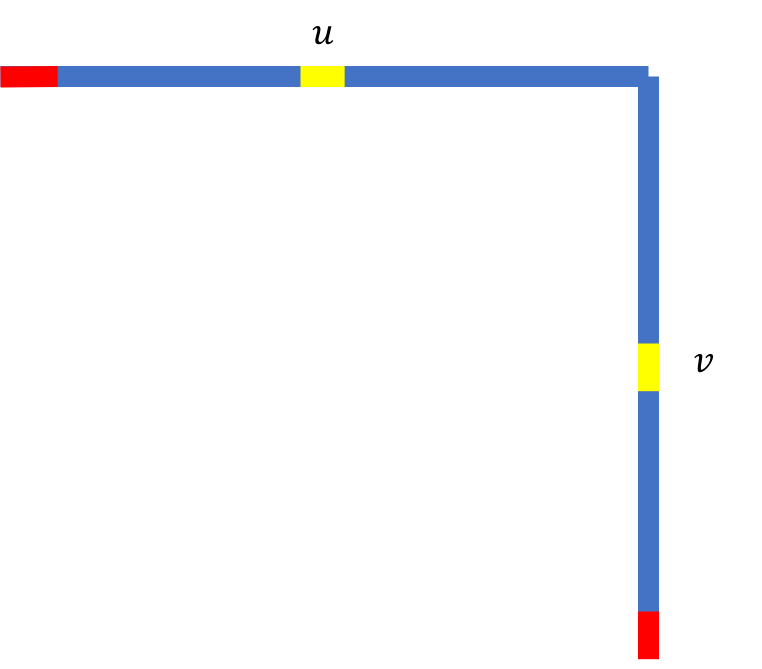
\includegraphics[scale=0.8]{ldmk_travel}
\centering
\caption{An example of different landmark travel time}\label{Fig:ldmk_travel}
\end{figure}

Imagine there are two landmarks $u$ and $v$, respectively, and each has a length of $L$ as shown in Figure~\ref{Fig:ldmk_travel}. Then, there are potentially infinite number of ways of `traveling from $u$ to $v$', because the starting point could be any points on $u$ and the ending point could be any points on $v$. If a driver starts at the red point on $u$ and stops at the red point on $v$, the total distance is $2L$ and the total time is $T$. But had the driver stopped at the yellow mid-point on $v$, the total distance would be $1.5L$ and the total time would be $3T/4$, assuming the speed is constant. 

Therefore, it is difficult to give a \emph{definite} estimate of the travel time between two landmarks. In this project, the \textbf{median travel time} is instead used to represent the travel time between two landmarks. It describes the \emph{typical} travel time a driver should expect. An example of a median case is that the diver starts at the yellow mid-point on $u$ and ends at the yellow mid-point on $v$. But there are in fact infinite number of median cases. 

The most significant 150 edges were selected to be evaluated, from \emph{each} of the four landmark graphs listed in Table~\ref{Ta:ldmkgraphs}. For each edge $(u, v)$, 20\% of the trajectories with $u$ as starting point and $v$ as ending point were randomly sampled. These trajectories represent some random trips between $u$ and $v$ with varying distances. Baidu Maps API was then used to estimate the travel time for each trajectory in real time, after which the median of all the estimates was selected as Baidu's estimate for the travel time between $u$ and $v$. Finally, Theorem~\ref{Theorem: weibull_inverse_dist} was used to calculate its own the travel time estimate which was then compared against Baidu's. Table~\ref{Ta:eval_res} summarises the evaluation results for all 150 significant edges. 

\begin{table}[h!]
\centering
\resizebox{\columnwidth}{!}{
\begin{tabular}{ | c | c | c | c |}
\hline
\textbf{Landmark Graph} & \textbf{RMSE} & \textbf{Mean Error Ratio} & \textbf{Mean No. of Samples Per Edge} \\ \hline
wrkd\_ldmkgraph\_50m & 78.84 & -0.009 & 1824.60 \\ \hline
wrkd\_ldmkgraph\_30m & 87.96 & -0.065 & 1507.56 \\ \hline
holi\_ldmkgraph\_50m & 87.39 & -0.16 & 832.96 \\ \hline
holi\_ldmkgraph\_30m & 76.41 & -0.14 & 681.89 \\ \hline
\end{tabular}}
\caption{Summary of Evaluation Results}\label{Ta:eval_res}
\end{table}

Assuming a Baidu's estimate is $b_{i}$ and the corresponding project's estimate is $\hat{b}_{i}$, then the Root Mean Square Error (RMSE) is given by:
\begin{equation}
RMSE = \sqrt{\frac{\sum_{i = 1}^{N}(\hat{b}_{i} - b_{i})^{2}}{N}}
\end{equation}
where $N$ is the total number of estimates; and the Mean Error Ratio (MER) is given by:
\begin{equation}
MER = \frac{1}{N}\sum_{i = 1}^{N}\frac{\hat{b}_{i} - b_{i}}{b_{i}}
\end{equation}

The RMSE gives an overall measure of accuracy. For instance, the RMSE for landmark graph \emph{wrkd\_ldmkgraph\_50m} turned out to be 78.58, which means that on average, the difference between Baidu's estimates and Theorem~\ref{Theorem: weibull_inverse_dist}'s estimate was 78.58 seconds. But whether this difference is significant or not depends on the scale of Baidu's estimates. For a Baidu's estimate of 30 seconds, 78.58 seconds may be considered significant, but for an estimate of 200 seconds, it may be acceptable. 

Therefore, MER is designed to take into account the scale of Baidu's estimates. It computes the ratio between the error and Baidu's estimate. A positive MER indicates that on average Theorem~\ref{Theorem: weibull_inverse_dist} tends to have larger estimates than Baidu's; on the other hand, a negative MER indicates that on average, Theorem~\ref{Theorem: weibull_inverse_dist} tends to have smaller estimates than Baidu's. 

Another technique to gauge Theorem~\ref{Theorem: weibull_inverse_dist}'s performance is linear regression. An ordered pair of estimates $(b_{i}, \hat{b}_{i})$ can be treated as a point in a 2-D Cartesian system. In the \emph{ideal} case, $\hat{b}_{i}$ should be equal to $b_{i}$, therefore, all points should form a straight line with a slope of 1 and an intercept of 0 when plotted. In the general cases, the regression equation gives the relationship between $b_{i}$ and $\hat{b}_{i}$. If the slope of the regression equation is less than 1, then $\hat{b}_{i}$ is expected to be less than $b_{i}$ in \emph{most} cases depending on the intercept. Figure~\ref{Fig:regression_plot} shows the regression plots. 

In summary, the estimates Theorem~\ref{Theorem: weibull_inverse_dist} gave were smaller than Baidu's estimates in most cases, which to some extent, was actually expected. The data set was collected in 2009 but Baidu Maps was giving \emph{real-time} estimates. Eight years since then, the travel time in the entire road network should have increased in general, due to increase in car ownership. Nevertheless, it still provides reasonable estimates with RMSE around 90 seconds. 

\begin{figure}[h!]
\begin{subfigure}{.5\textwidth}
\centering
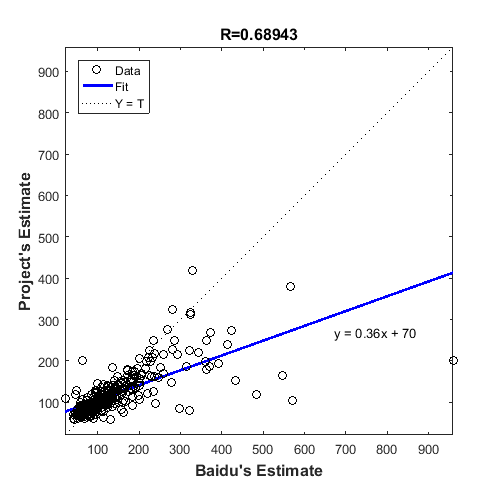
\includegraphics[width = .9\linewidth]{wrkd_50m_reg}
\caption{wrkd\_ldmkgraph\_50m}
\label{Fig:wrkd_50m_reg}
\end{subfigure}
\begin{subfigure}{.5\textwidth}
\centering
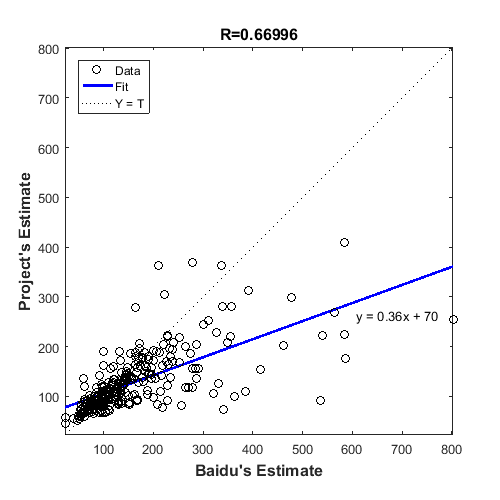
\includegraphics[width = .9\linewidth]{wrkd_30m_reg}
\caption{wrkd\_ldmkgraph\_30m}
\label{Fig:wrkd_30m_reg}
\end{subfigure}

\begin{subfigure}{.5\textwidth}
\centering
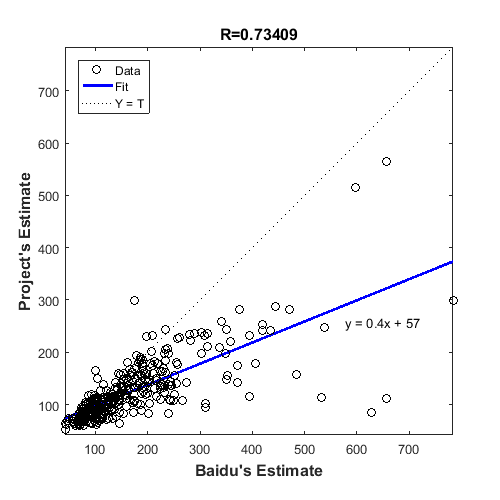
\includegraphics[width = .9\linewidth]{holi_50m_reg}
\caption{holi\_ldmkgraph\_50m}
\label{Fig:holi_50m_reg}
\end{subfigure}
\begin{subfigure}{.5\textwidth}
\centering
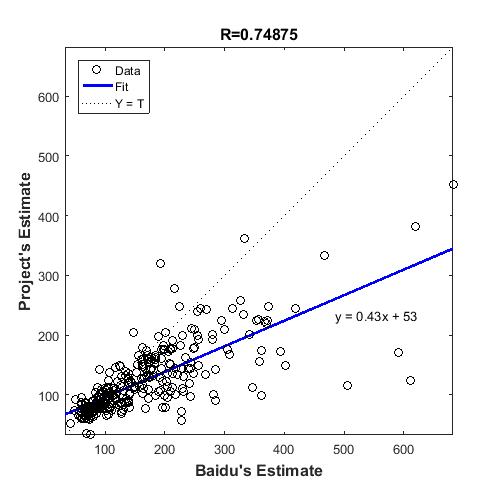
\includegraphics[width = .9\linewidth]{holi_30m_reg}
\caption{holi\_ldmkgraph\_30m}
\label{Fig:holi_30m_reg}
\end{subfigure}

\caption{Regression Plots}
\label{Fig:regression_plot}
\end{figure}



\appendix
\chapter{Source Code}
\section{Database Utilities}
The source code listed in this section provides utility functions for general database operations, such as \textbf{select} and \textbf{update}. It is to be used in other modules. 

\begin{lstlisting}[language = PHP, caption = {Database Utilities}, label = {AList:db_utilities}, frame=single, numbers=left, stepnumber=1]
<?php
include "../inc/jingodbinfo.inc";

function connect_db(){
    $conn = new mysqli(DB_SERVER, DB_USERNAME, DB_PASSWORD);
    if($conn->connect_error){
	die("Connection failed: " . $conn->connect_error);
    }
    $conn->select_db(DB_DATABASE);
    $conn->set_charset("utf8");
    return $conn;
}

function disconnect_db($conn){ $conn->close(); }

function db_select($conn, $table, $cols, $cond = "true", $distinct = "")
{
    $sql_select = "SELECT {$distinct} ";
    if(count($cols) == 0){
        $sql_select .= "*,";
    }
    foreach ($cols as $col) {
        $sql_select .= "{$col},";
    }
    $sql_select = rtrim($sql_select, ",");
    $sql_select .= " FROM {$table} WHERE {$cond};";
    $ret = $conn->query($sql_select);
    $res = array();
    if($ret->num_rows > 0){
        while($row = $ret->fetch_assoc()){
            $curr = array();
            foreach ($cols as $col) {
                $curr[$col] = $row[$col];
            }
            $res[] = $curr;
	}
    }
    return $res;
}

function db_update($conn, $table, $values, $cond){
    $sql_update = "UPDATE {$table} SET ";
    foreach ($values as $key => $value) {
        if(is_numeric($value)){
            $sql_update .= "{$key} = {$value},";
        }else{
            $sql_update .= "{$key} = '{$value}',";
        }
    }
    $sql_update = rtrim($sql_update, ",");
    $sql_update .= " WHERE {$cond};";
    $succ = $conn->query($sql_update);
    return $succ;
}

function db_insert($conn, $table, $values, $cond = "", $ignore = ""){
    $sql_insert = "INSERT {$ignore} INTO {$table} ";
    $cols = "";
    $vals = "";
    foreach ($values as $key => $value) {
        $cols .= "{$key},";
        $vals .= (is_numeric($value) ? "{$value}," : "'{$value}',");
    }
    $cols = rtrim($cols, ",");
    $vals = rtrim($vals, ",");
    $sql_insert .= "({$cols}) VALUES ({$vals}) {$cond};";
    echo "{$sql_insert}\n";
    $conn->query($sql_insert);
}

function db_delete($conn, $table, $cond){
    $sql_delete = "DELETE FROM {$table} WHERE {$cond};";
}
?>
\end{lstlisting}

\clearpage
\newpage

\section{Data Pre-processing}
This section lists down the source code used in data pre-processing. 

\begin{lstlisting}[language = PHP, caption = {Outlier Removal}, label = {AList:outlier_rmvl}, frame=single, numbers=left, stepnumber=1]
<?php
include "db_utilities.php";

class Filter{
    private $ldmk_start;
    private $ldmk_end;
    private $ldmk_table;
    private $data_table;
    private $update_table;
    private $path;
    private $bchmk;
    
    private $conn;
    private $num_dele;
    
    public function __construct($ldmk_start, $ldmk_end, $ldmk_table, $data_table, $path, $bchmk, $update_table){
        $this->ldmk_start = $ldmk_start;
        $this->ldmk_end = $ldmk_end;
        $this->ldmk_table = $ldmk_table;
        $this->data_table = $data_table;
        $this->update_table = $update_table;
        $this->path = $path;
        $this->bchmk = $bchmk;
        $this->conn = connect_db();
        $this->num_dele = 0;
    }
    
    public function __destruct(){ disconnect_db($this->conn); }
    
    private function getCentres($ldmk){
        $filename = "{$this->path}{$ldmk}.csv";
        $centres = array();
        if(($handle = fopen($filename, 'r')) !== FALSE){
            while(($line = fgetcsv($handle, 0, ',')) !== FALSE){
                $centres[] = array($line[0], $line[1]);
            }
	}
	return $centres;
    }
    
    private function getRecords($ldmk){
        $ldmk_cols = array('LandmarkName');
        $ldmk_cond = "LandmarkID = {$ldmk}";
        $ret = db_select($this->conn, $this->ldmk_table, $ldmk_cols, $ldmk_cond);
        $data_cols = array('DataUnitID', 'BD09_LONG', 'BD09_LAT');
        $data_cond = "Street = '{$ret[0][$ldmk_cols[0]]}'";
        $ret = db_select($this->conn, $this->data_table, $data_cols, $data_cond);
        $records = array();
        foreach ($ret as $item) {
            $records[] = array($item[$data_cols[0]], $item[$data_cols[1]], $item[$data_cols[2]]);
        }
        return $records;
    }
    
    
    private function removeRecord($centres, $records){
        foreach ($records as $recd) {
            $min_dist = INF;
            foreach ($centres as $centre) {
                $min_dist = min($min_dist, $this->getHaversineDist
                ($centre[0], $centre[1], $recd[1], $recd[2]));
            }
            if($min_dist > $this->bchmk){
                $cond = "DataUnitID = {$recd[0]}";
                db_delete($this->conn, $this->data_table, $cond);
                ++$this->num_dele;
            }
	}
    }
    
    private function toRadian($degree){ return $degree * M_PI / 180; }
    
    private function getHaversineDist($long1, $lat1, $long2, $lat2){
        $BJ_LAT = $this->toRadian(39);
        $EQ_R = 6378137; // equatorial radius in metres
        $POL_R = 6356752; // polar radius in metres

	$BJ_R = sqrt((pow($EQ_R * $EQ_R * cos($BJ_LAT), 2) + pow($POL_R * $POL_R * sin($BJ_LAT), 2)) / (pow($EQ_R * cos($BJ_LAT), 2) + pow($EQ_R * sin($BJ_LAT), 2)));
	$long1 = $this->toRadian($long1);
	$lat1 = $this->toRadian($lat1);
	$long2 = $this->toRadian($long2);
	$lat2 = $this->toRadian($lat2);
	$d = 2 * $BJ_R * asin(sqrt(pow(sin(($lat1 - $lat2) / 2), 2) + 
	cos($lat1) * cos($lat2) * pow(sin(($long1 - $long2) / 2), 2)));
	return $d; }
    private function getWithin($ldmk, $centres, $records){
        foreach ($records as $recd) {
	    $min_dist = INF;
	    foreach ($centres as $centre) {
	        $min_dist = min($min_dist, 
		$this->getHaversineDist($centre[0], $centre[1], $recd[1], $recd[2]));
	    }
	    if($min_dist <= $this->bchmk){
	        db_insert($this->conn, $this->update_table, 
			array('LandmarkID' => $ldmk, 'BD09_LONG' => $recd[1], 'BD09_LAT' => $recd[2]));
	    }
	}
    }
    
    public function doFiltering(){
	for($ldmk = $this->ldmk_start; $ldmk != $this->ldmk_end; 
		++$ldmk){
	    $centres = $this->getCentres($ldmk);
	    $records = $this->getRecords($ldmk);
	    $this->getWithin($ldmk, $centres, $records);
	}
    }
}
set_time_limit(0);
ini_set('memory_limit','2048M');
$filter = new Filter($_POST['ldmk_start'], $_POST['ldmk_end'], 
	$_POST['ldmk_table'], $_POST['data_table'], $_POST['path'], 
	$_POST['bchmk'], $_POST['update_table']);
$filter->doFiltering();
?>
\end{lstlisting}

%\chapter{Figures}

\vspace*{-3in}

\begin{figure}
\vspace{2.4in}
\caption{Armadillo slaying lawyer.}
\label{arm:fig1}
\end{figure}
\clearpage
\newpage

\begin{figure}
\vspace{2.4in}
\caption{Armadillo eradicating national debt.}
\label{arm:fig2}
\end{figure}
\clearpage
\newpage

%\bibliography{main}
%\bibliographystyle{alpha}
%% This defines the bibliography file (main.bib) and the bibliography style.
%% If you want to create a bibliography file by hand, change the contents of
%% this file to a `thebibliography' environment.  For more information 
%% see section 4.3 of the LaTeX manual.
\begin{singlespace}
\bibliography{main}
\bibliographystyle{plain}
\end{singlespace}

\end{document}

